\chapter{聚类}
\label{chap:clustering}

客户记录没有类别标签时，消费金额相近的人未必购买相同品类，购买品类相近的人也未必有相同频率。\term{聚类}（clustering）先选定要保留的相似关系，再据此寻找群组；这项选择决定了“同一簇”的含义。给定$\bm{x}_1,\ldots,\bm{x}_n\in\mathbb{R}^{d}$，硬划分记为$\mathcal{P}=\{C_1,\ldots,C_K\}$，其中$C_k$是样本索引集合，$c_i=k$表示$i\in C_k$。通常要求簇非空、互斥且覆盖全部样本；噪声、重叠和软归属方法则采用各自的输出约定。

1950至1960年代，中心划分与层次聚类逐渐形成，K-means成为代表方法。1990年代的数据挖掘推动了DBSCAN等密度方法及大规模、子空间聚类；谱方法则从图关系理解群组。概率混合思想有更早的统计来源，19世纪末已用于分析异质总体\scite{clust-macqueen1967,ester1996,clust-pearson1894}。

所需输出可以帮助缩小方法范围。大样本的数值分组和量化可采用K-means及小批量更新；弯曲的密集区域和噪声识别可采用DBSCAN或HDBSCAN；嵌套粒度与成分后验则分别由层次方法和混合模型提供。比较时还需核对距离、密度尺度与分布假设是否符合数据\scite{classic-clustering-guide}。

本章按构造群组的机制展开。原型方法比较样本与代表，邻域和图方法利用连接，网格与子空间方法寻找局部相关结构，层次方法保留嵌套分组，概率方法推断成分归属，集成方法汇总多份划分，半监督方法再加入领域信号。各机制承接第\ref{chap:classic-models-overview}章，也可以共同用于一个模型。

\section{基于原型的聚类}
\label{sec:clustering-partition}

把客户分成 $K$ 组时，可以为每组选择一个代表，并用样本到代表的相异度衡量分组质量。原型聚类最小化这些簇内相异度的总和；各代表竞争样本，形成不同的分配区域。这里的直接目标是组内拟合，簇间分离由分配规则间接产生。

K-means 用均值表示簇，计算方便；K-medoids 用真实样本表示簇，能够使用更一般的相异度。两者共享分配与代表选择的思路，但优化变量和求解方法不同。

\subsection{K-means}
\label{sec:clustering-kmeans}

若样本是数值向量，均值是一个自然的代表：它综合了簇内所有样本的位置。\term{K均值聚类}（K-means）据此寻找 $K$ 个中心，使样本到所属中心的平方距离之和尽量小。

K-means的目标与更新算法来自多项研究。Steinhaus的《论物质体的分割》刊于第4卷第12期，卷册标为1956年，zbMATH按1957年著录\scite{clust-steinhaus1957}。MacQueen在1967年使用K-means这一名称，讨论逐个吸收样本并立即调整均值的增量算法\scite{clust-macqueen1967}。因此，文献中的K-means有时指平方误差目标，有时指具体求解过程；两种用法需结合更新步骤识别。

本节采用Lloyd的批量更新。它源于信号量化：把连续幅值映射为有限代表值，并控制平方失真。相关工作完成于1957年，经典论文于1982年正式发表\scite{clust-lloyd1982}。Lloyd交替执行最近代表分配与均值重估，每轮使用完整样本；MacQueen则在读入一个样本后立即更新。常见批量实现沿用前一种过程。

平方距离与均值更新使两个条件子问题都容易计算，一轮分配和更新约需 $O(nKd)$ 运算。K-means由此可用于用户分群、向量量化和图像颜色压缩，也可承担谱聚类的离散化或混合模型的初始化。具体用途仍需明确平方失真所代表的损失。

\subsubsection{模型结构}

为第 $k$ 个簇配置中心 $\bm{\mu}_k\in\mathbb{R}^d$，其\term{簇内平方误差}（sum of squared errors, SSE）为
\begin{equation}
  J(\mathcal{P},\bm{\mu})
  =\sum_{k=1}^K\sum_{i\in C_k}
    \lVert\bm{x}_i-\bm{\mu}_k\rVert_2^2.
  \label{eq:clustering-sse}
\end{equation}
这里 $\bm{\mu}=(\bm{\mu}_1,\ldots,\bm{\mu}_K)$ 表示中心参数。固定中心后，每个样本应归入距离最近的中心；固定分配后，每个中心应取簇内均值。

平方欧氏距离的等距离面是球面，最近中心的分配区域是由超平面分隔的Voronoi单元。这样的表示适合在中心附近紧凑分布的群组，环形等非凸群组可能被多个中心拆开。簇的尺度差异也会影响中心数的分配；这些限制来自几何准则，无需假定样本严格服从球形高斯。

\subsubsection{参数学习}

同时优化中心和分配较难，但两个条件子问题都可直接求解。记第 $t$ 轮的分配为 $c_i^{(t)}$，Lloyd 更新写为
\begin{align}
  c_i^{(t+1)}
    &\in\argmin_{1\leq k\leq K}
      \lVert\bm{x}_i-\bm{\mu}_k^{(t)}\rVert_2^2,
      \label{eq:clustering-lloyd-assignment}\\
  \bm{\mu}_k^{(t+1)}
    &=\frac{1}{|C_k^{(t+1)}|}
      \sum_{i\in C_k^{(t+1)}}\bm{x}_i.
      \label{eq:clustering-lloyd-centre}
\end{align}
图~\ref{fig:clustering-lloyd-steps}固定六个样本，分别展示分配与中心更新的作用。中图只重算中心，保留左图的簇标记；右图再比较距离，样本$(1,0)$才由方块簇转入圆点簇。把这两个动作分开展示，才能分别核对每个条件子问题怎样降低目标。

\Needspace{65mm}
\begin{figure*}[htbp]
  \centering
  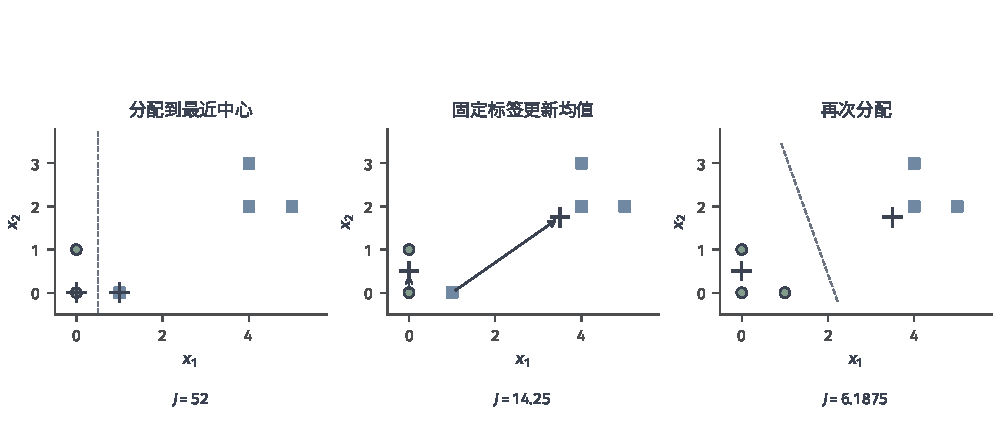
\includegraphics[width=159.059mm]{figures/04-classic-models/00-shared/matplotlib/clustering-lloyd-steps/figure.pdf}
  \caption{Lloyd 迭代的教学例，六个样本为 $(0,0)$、$(0,1)$、$(1,0)$、$(4,2)$、$(4,3)$、$(5,2)$，初始中心为 $(0,0)$ 和 $(1,0)$。圆点与方块表示两个簇，十字表示中心，虚线表示等距边界。首次更新后中心为 $(0,0.5)$ 和 $(3.5,1.75)$；图中依次展示分配、均值更新与再次分配。}
 \label{fig:clustering-lloyd-steps}
\end{figure*}

平局与空簇需要纳入更新规则。等距时优先保留仍属最优的原分配，初始化则按固定顺序决定；空簇没有均值，下面保留其旧中心。这一教学实现最多返回$K$个非空簇。要求恰好$K$个非空簇时，可采用重启或后文的容量约束，并核对相应的停止条件。

\begin{codeblock}[language=Python,label={code:clustering-kmeans}]{带平局与空簇处理的 Lloyd 迭代}
import numpy as np

def kmeans(X, K, max_iter=300, seed=0):
    X = np.asarray(X, dtype=float)
    n = len(X)
    if not 1 <= K <= n or max_iter < 1:
        raise ValueError("invalid K or max_iter")
    rng = np.random.default_rng(seed)
    mu = X[rng.choice(n, K, replace=False)].copy()
    labels = np.full(n, -1)
    for _ in range(max_iter):
        d2 = ((X[:, None] - mu[None]) ** 2).sum(2)
        new = d2.argmin(1)
        rows = np.flatnonzero(labels >= 0)
        keep = d2[rows, labels[rows]] == d2[rows, new[rows]]
        new[rows[keep]] = labels[rows[keep]]
        if np.array_equal(new, labels):
            return labels, mu
        labels = new
        for k in range(K):
            members = X[labels == k]
            if len(members):
                mu[k] = members.mean(0)
    return labels, mu
\end{codeblock}

代码接受有限的二维数值数组。正常停止时，分配与中心形成不动点；迭代上限提前触发时，返回中心已按当前分配更新，但这些分配可能还需再比较一次最近中心。两种退出情形应分别记录。广播计算临时占用$O(nKd)$空间，样本较多时可分块计算距离。

初始中心决定Lloyd从哪里开始搜索。\term{K-means++}先均匀选一个样本，再按$D_i^2/\sum_jD_j^2$抽取后续中心，其中$D_i$是样本到已有中心的最近距离。所有$D_i=0$时，已有中心已覆盖全部不同位置。Arthur与Vassilvitskii证明了初始目标的期望界$\mathbb{E}[J]\leq8(\log K+2)J^\ast$；Lloyd后续不增目标，因此保留这一界\scite{clust-arthur2007}。

该界平均了初始化随机性，单次运行的结果仍可能相差较大。标准K-means++逐个选中心，约需$O(nKd)$运算；分布式实现还需计入数据扫描与通信。评价初始化时，可以同时比较最终平方误差、重启次数和总成本。

\subsubsection{理论分析}

\paragraph{表达能力}
K-means以最近中心的Voronoi区域表示分组，适合按平方距离集中在中心附近的簇。弯曲、尺度差异很大或由其他相异度定义的簇可能不在这个表示偏好内。

\paragraph{收敛性}
Lloyd的有限停止需要目标下降与平局规则共同支持。目标有下界且不增，足以得到目标值的极限；进一步排除无穷次分配变化，才可得到有限轮停止。下面利用有限分配集合完成这一步。

\begin{theorem}[Lloyd 算法的单调性与有限停止]
  \label{thm:clustering-lloyd}
  对有限样本，在精确计算下，分配步采用最近中心规则，并在平局时优先保留原簇分配；更新步对非空簇取均值、对空簇保留旧中心。则目标值单调不增，算法在有限轮后到达分配和中心均不再变化的不动点。
\end{theorem}
\begin{proof}
固定中心，逐点选择最小距离给出
\[
 J(\mathcal{P}^{(t+1)},\bm{\mu}^{(t)})
 \leq J(\mathcal{P}^{(t)},\bm{\mu}^{(t)}).
\]
对任意非空簇 $C$，记均值为 $\bar{\bm{x}}_C$。展开平方项，并利用 $\sum_{i\in C}(\bm{x}_i-\bar{\bm{x}}_C)=\bm{0}$，得到
\begin{equation}
 \sum_{i\in C}\lVert\bm{x}_i-\bm{a}\rVert_2^2
 =\sum_{i\in C}\lVert\bm{x}_i-\bar{\bm{x}}_C\rVert_2^2
   +|C|\lVert\bm{a}-\bar{\bm{x}}_C\rVert_2^2.
 \label{eq:clustering-mean-decomposition}
\end{equation}
所以均值是唯一最优中心，更新步也不会增加目标；空簇对目标贡献为零。

第一次均值更新后，若分配改变，至少一个样本移向严格更近的中心，否则保留原标签的规则会阻止改变。因此完整一轮使目标严格下降。对任一分配，均值更新后的目标只由该分配决定，即使存在空簇也如此。分配至多有 $K^n$ 种，严格下降不可能无限次访问它们。分配不变时，已有非空簇中心仍为相同均值，算法遂停止。
\end{proof}

不动点在固定中心时满足最近分配，在固定分配时满足均值最优。若每个样本的最近中心唯一、各簇非空，则足够小的中心扰动保持分配，均值最优性给出局部最优解释。等距样本或重合中心可能破坏这一局部稳定条件，需按退化结构分析。

两个子问题易解，联合的全局搜索仍可能昂贵。维数属于输入时，固定$K=2$的欧氏平方和聚类已是NP-hard\scite{clust-aloise2009}。平面上将$K$作为输入也有NP-hard结果\scite{clust-mahajan2012}。这些结果表明，在$\mathrm{P}\ne\mathrm{NP}$的前提下，一般输入的精确全局解无法统一用多项式时间取得。

\paragraph{泛化性}
未来样本$\bm{X}$与训练样本同分布时，可用总体量化误差$\mathbb{E}[\min_k\lVert\bm{X}-\bm{\mu}_k\rVert_2^2]$评价所学中心。经验全局最优中心在矩条件和适当唯一性条件下具有一致性理论\scite{clust-pollard1981}。一次Lloyd运行得到的是某个不动点，应用该理论还需核对其与经验全局解的关系。

输入表示同样影响量化误差。平方距离放大远离中心的样本，不同量纲改变最近中心的次序，因此尺度选择需对应业务含义。第\ref{sec:regression-knn}节的$k$-NN回归也依赖距离，但它平均带响应的邻居，K-means则拟合无标签输入的位置。重启改变搜索起点；修改相似度或模型改变所表达的结构，二者处理不同来源的误差。

\subsubsection{支持大规模数据（Mini-Batch K-means）}

样本量较大时，一轮全量扫描也可能超过更新预算。Sculley在2010年提出\term{小批量K均值聚类}（Mini-Batch K-means），每轮抽取$b$个样本，只调整它们涉及的中心\scite{clust-sculley2010}。

设簇 $k$ 累计接收了 $v_k$ 次样本更新。每接收一个分配到该簇的样本，就令 $v_k\leftarrow v_k+1$，并计算
\begin{equation}
 \bm{\mu}_k\leftarrow
 (1-\eta_k)\bm{\mu}_k+\eta_k\bm{x}_i,
 \qquad \eta_k=\frac{1}{v_k}.
 \label{eq:clustering-minibatch}
\end{equation}
这是对历史已分配样本的增量平均，不是当前全体簇成员的精确均值。一轮距离计算降为 $O(bKd)$，但总成本仍取决于迭代次数、初始化和最终全量分配。

随机小批量使每次更新只反映部分样本，逐轮全量SSE可能波动。批量大小、采样偏差和低频簇的覆盖影响最终误差；定理~\ref{thm:clustering-lloyd}针对完整分配与精确均值更新，其单调性前提在这里发生改变。选择计算预算时，应以抽样评价或留出量化误差检查这种近似是否足够。

\subsubsection{支持限制簇大小（Constrained K-means）}
\label{sec:clustering-capacity}

最小 SSE 不一定满足容量需求。客户分区、任务分片或服务网点分配常要求每簇至少或至多容纳一定数量的样本。Bradley、Bennett 与 Demiriz 研究了带最小簇规模的 K-means；加入上界后，固定中心的分配问题可统一写为\scite{clust-bradley2000}。
\begin{equation}
 \begin{aligned}
 \min_{\bm{Z}}\quad&
   \sum_{i=1}^n\sum_{k=1}^K
   z_{i,k}\lVert\bm{x}_i-\bm{\mu}_k\rVert_2^2,\\
 \text{s.t.}\quad&
   \sum_{k=1}^K z_{i,k}=1,\quad z_{i,k}\in\{0,1\},\\
 & \ell_k\leq\sum_{i=1}^n z_{i,k}\leq u_k.
 \end{aligned}
 \label{eq:clustering-capacity}
\end{equation}
整数容量满足 $0\leq\ell_k\leq u_k$，且在没有其他分配禁令时，可行性条件为 $\sum_k\ell_k\leq n\leq\sum_ku_k$。

固定中心的容量分配可转为最小费用流。源点到每个样本的边容量为1，样本到每簇的边容量为1、费用为平方距离，簇到汇点的边下界为$\ell_k$、上界为$u_k$，总流量为$n$。网络流的整数性保证存在整数最优解，使每个样本恰好选择一簇；这一性质来自网络约束的结构。

容量方法的中心仍按均值更新。每次分配精确最优且平局保留已有最优分配时，分配变化导致严格下降；采用确定的空簇处理后，可按有限分配集合证明停止。求解成本取决于网络规模、费用表示与求解器，需按具体实现估计。

Malinen 与 Fränti 在 2014 年研究了要求簇规模相等的平衡 K-means\scite{clust-malinen2014}。当 $K$ 整除 $n$ 且要求 $|C_k|=n/K$ 时，把每个中心复制成相应数量的容量槽，得到 $n$ 对 $n$ 的指派问题；Hungarian 算法可在 $O(n^3)$ 时间内求解。

当$n$不能被$K$整除，可为各簇指定$\lfloor n/K\rfloor$或$\lceil n/K\rceil$个槽，并使容量总和为$n$。按距离顺序填槽可以节省搜索，却可能让先处理的样本占用后续样本所需位置。使用这种启发式时，还需检查全部下界与实际SSE变化。

\subsubsection{小结}

K-means将数值硬划分写成平方失真最小化，计算便利来自最近中心与均值两个可解子问题。尺度、离群点、初始化和$K$决定实际划分；Mini-Batch减少每次更新的数据量，容量约束限制可行分配。两种扩展改变计算或约束，中心几何仍沿用原模型。

\subsection{K-medoids}
\label{sec:clustering-kmedoids}

解释客户群组时，可能希望给出一条真实记录；对字符串等对象，均值也缺乏定义。\term{K 中心样本聚类}（K-medoids）从观测对象中选代表，只依赖样本之间的相异度，因而可在这些场景中使用。

Kaufman与Rousseeuw在1987年介绍了通过medoid聚类的方法，以真实观测作代表，使相异度矩阵能够直接作为输入\scite{clust-kaufman1987}。1990年的专著进一步整理了PAM、面向较大数据的CLARA及层次分析\scite{clust-kaufman1990}。代表的解释与候选代表的搜索由此成为两个独立的设计问题。

\subsubsection{模型结构}

设代表索引集合 $M=\{m_1,\ldots,m_K\}\subseteq\{1,\ldots,n\}$，相异度为 $\delta(\bm{x},\bm{y})$。优化目标为
\begin{equation}
 J(M)=\sum_{i=1}^n\min_{m\in M}\delta(\bm{x}_i,\bm{x}_m).
 \label{eq:clustering-medoids}
\end{equation}
每个 $\bm{x}_{m_k}$ 称为\term{中心样本}（medoid），分配由最近代表决定。典型相异度包括欧氏距离、曼哈顿距离、汉明距离、编辑距离和 Jaccard 距离。目标本身不要求三角不等式，但某些索引加速方法需要这一性质。

未平方距离随远点的偏移增长较慢，真实样本约束也改变了中心的可移动范围，两者可减弱极端值对SSE均值的影响。具体鲁棒性仍由相异度和污染位置决定：离群点若改变候选代表的相对距离，也可能改变medoid。

图~\ref{fig:clustering-medoid-robustness}固定一维单簇，将最右样本由5移到12。平方距离的最优中心随均值右移，绝对距离的最优中心样本仍为中间观测2。该对照同时改变损失与代表约束，结论限于这组设定；它提供了检查极端值影响的可核算例子。

\Needspace{75mm}
\begin{figure}[htbp]
  \centering
  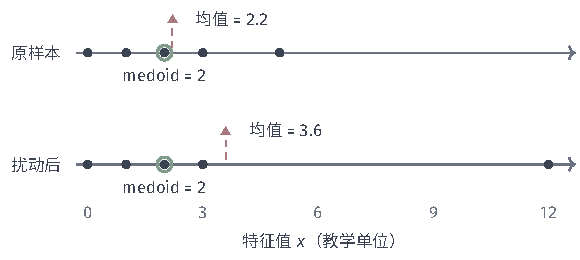
\includegraphics[width=98.231mm]{figures/04-classic-models/00-shared/tikz/clustering-medoid-robustness/figure.pdf}
  \caption{中心样本与均值对极端值的不同反应。固定 $K=1$，上方样本为 $\{0,1,2,3,5\}$，下方只把 5 改为 12；黑点为观测，圆圈标出绝对距离下的 medoid，三角形标出平方距离下的最优均值。}
 \label{fig:clustering-medoid-robustness}
\end{figure}

\subsubsection{参数学习}

\term{围绕中心样本划分}（Partitioning Around Medoids, PAM）通常包含 BUILD 初始化和 SWAP 改进。BUILD 贪心增加代表；SWAP 枚举每个当前代表 $m\in M$ 与每个非代表 $o\notin M$，计算
\[
 \Delta(m,o)=
 J\bigl((M\setminus\{m\})\cup\{o\}\bigr)-J(M).
\]
候选 $o$ 来自整个数据集，而不限于 $m$ 所在簇；每次交换后，所有样本都重新选择最近代表。只在固定簇内选取距离总和最小的样本，是另一种交替更新，不能替代 PAM 的 SWAP。

下面从随机代表开始，逐个评价完整交换邻域，以便核对$J(M)$与返回状态。代码省略BUILD初始化和距离差分缓存，适合作为目标及停止判据的教学实现。

\begin{codeblock}[language=Python,label={code:clustering-pam}]{PAM 的完整交换步骤}
import numpy as np

def pam_swap(D, K, seed=0, max_iter=100):
    n = len(D)
    if D.shape != (n, n) or not 1 <= K <= n or max_iter < 1:
        raise ValueError("invalid distance matrix, K, or max_iter")
    rng = np.random.default_rng(seed)
    medoids = rng.choice(n, K, replace=False)
    cost = D[:, medoids].min(1).sum()
    converged = False
    for _ in range(max_iter):
        best, best_cost = None, cost
        outside = np.setdiff1d(np.arange(n), medoids)
        for k in range(K):
            for o in outside:
                trial = medoids.copy()
                trial[k] = o
                value = D[:, trial].min(1).sum()
                if value < best_cost:
                    best, best_cost = trial, value
        if best is None:
            converged = True
            break
        medoids, cost = best, best_cost
    return D[:, medoids].argmin(1), medoids, converged
\end{codeblock}

完整扫描若未发现改进交换，代码返回\code{converged=True}，表明当前代表集合在单次交换邻域中局部最优。迭代上限先触发时，\code{converged=False}保留了尚未核完下一邻域的状态。严格下降使代表集合不重复，去掉上限并继续扫描时，有限候选集合保证最终停止。

预计算相异度矩阵占用$O(n^2)$存储，距离本身的计算还需另外计入。经典PAM缓存最近与次近代表，一轮完整交换通常按$O(K(n-K)^2)$量级分析。教学代码为每个候选重算$K$个距离列，额外重复了这些访问，因此成本更高。

完整交换邻域昂贵时，CLARA在若干子样本上运行PAM，再用全体样本评价候选代表，以减少工作集和内存；小簇可能因抽样而遗漏。CLARANS把代表集合视为状态，随机抽取交换邻居，减少每轮扫描量\scite{clust-nghan1994}。两者分别近似候选来源与搜索邻域。

FastPAM复用不同被替换代表之间的计算，消除经典交换步骤中重复的$K$项工作，主要获得约$K$因子的加速\scite{clust-schubert2019}。关于$n$的距离访问和全量矩阵存储仍需计入，大样本的瓶颈可能继续来自这两部分。

\subsubsection{小结}

K-medoids以真实代表和一般相异度扩展原型聚类的输入与解释方式。与平方距离K-means比较时，极端值影响需结合所选损失；完整交换搜索和距离矩阵则带来额外计算。CLARA、CLARANS和FastPAM改变不同操作，可按允许的近似误差及内存预算选择。

\subsection{模型对比与总结}

原型方法可分别改变代表约束、损失、输出或表示。K-means的代表在向量空间中移动，目标是平方欧氏距离；K-medoids从观测中选代表，目标采用指定相异度。表~\ref{tab:clustering-partition}按这两个差异比较计算和用途，再讨论各方向的扩展。

\begin{table}[htbp]
 \small
 \begin{tabularx}{\linewidth}{@{}l>{\RaggedRight\arraybackslash}X>{\RaggedRight\arraybackslash}X@{}}
 \toprule
 比较项 & K-means & K-medoids\\
 \midrule
 代表 & 簇内均值向量 & 真实样本\\
 准则 & 平方欧氏距离和 & 指定相异度和\\
 优化步骤 & 最近中心与均值更新 & 代表交换与全局重分配\\
 主要成本 & 一轮 $O(nKd)$ & 完整交换搜索与距离访问\\
 典型用途 & 数值数据、向量量化 & 非数值对象、实例解释\\
 \bottomrule
 \end{tabularx}
 \caption{两类划分方法的比较。复杂度须与具体算法相联系；PAM 的成本不能套到所有 K-medoids 求解器。}
 \label{tab:clustering-partition}
\end{table}

沿中心与相异度两个方向，可以得到其他划分模型。\term{K 中位数聚类}（K-medians）最小化 $\ell_1$ 距离和，固定分配后逐坐标取中位数；它不等于以欧氏距离和定义的几何中位数问题。

\Needspace{45mm}
若簇之间允许模糊重叠，\term{模糊 C 均值}（Fuzzy C-Means, FCM）用隶属度 $u_{i,k}$ 代替硬簇分配\scite{clust-bezdek1981}。
\begin{equation}
 J_{\mathrm{FCM}}
 =\sum_{i=1}^n\sum_{k=1}^K
 u_{i,k}^{q}\lVert\bm{x}_i-\bm{\mu}_k\rVert_2^2,
 \quad \sum_k u_{i,k}=1,\quad q>1.
 \label{eq:clustering-fcm}
\end{equation}
这里$q$控制隶属度的模糊程度。固定隶属度时，中心是以 $u_{i,k}^q$ 为权重的均值；当各距离非零时，固定中心给出
\[
 u_{i,k}=
 \left[
 \sum_{j=1}^K
 \left(\frac{\lVert\bm{x}_i-\bm{\mu}_k\rVert_2}
 {\lVert\bm{x}_i-\bm{\mu}_j\rVert_2}\right)^{2/(q-1)}
 \right]^{-1}.
\]
若样本与一个或多个中心重合，可把隶属度集中在这些零距离中心上。隶属度表示模糊目标下的软归属；赋予生成后验含义还需要相应概率模型。医学影像中一个像素混合多种组织的部分体积效应，可为这种软表达提供应用动机。

\term{二分 K-means}（Bisecting K-means）改变分裂顺序：先把全部样本放在一簇，再反复选择一个簇作$K=2$划分。常见实现选择最大SSE的簇，并为每次二分多次重启。它形成层次结构，早期分裂限制后续分组，因此最终SSE应与同条件的一次性$K$分比较。Steinbach等在文档聚类中研究了这一方案\scite{clust-steinbach2000}。

% 将核距离推导及两条较长的引文安排在同一段版面内。
\Needspace{105mm}
若主要困难是原空间中的非凸形状，可在特征映射 $\phi$ 后运行\term{核 K-means}（kernel K-means）。使用第\ref{sec:classic-overview-kernel-trick}节定义的正定核$K$，本节只需把簇内平方距离改为特征空间距离。样本到簇均值的平方距离为
\begin{equation}
 \begin{aligned}
 \lVert\phi(\bm{x}_i)-\bm{\mu}_k^\phi\rVert^2
 ={}&K(\bm{x}_i,\bm{x}_i)
 -\frac{2}{|C_k|}\sum_{j\in C_k}K(\bm{x}_i,\bm{x}_j)\\
 &+\frac{1}{|C_k|^2}
   \sum_{j,l\in C_k}K(\bm{x}_j,\bm{x}_l).
 \end{aligned}
 \label{eq:clustering-kernel-kmeans}
\end{equation}
公式只使用核值，省去了显式构造$\phi$，相应成本转为核矩阵计算与存储\scite{clust-girolami2002,dhillon2004}。Girolami讨论核空间聚类，Dhillon、Guan与Kulis进一步联系了适当权重和核构造下的核K-means与归一化割。

核K-means与归一化割的联系依赖适当的权重和核构造，适用范围需随具体等价关系核对。特征映射可以改变原空间的分配形状，层次结构则改变输出粒度。第\ref{sec:clustering-hierarchy}节再讨论多层输出，下面先利用局部密度和连接描述弯曲群组。

\section{基于邻域的聚类}
\label{sec:clustering-density}

环形、月牙形和弯曲条带中的样本可能远离同一中心，却能沿密集区域连接。密度方法据此把低密度分隔加入簇定义：一类方法寻找密集区域的连通分量，另一类寻找密度峰的吸引域。同一连通区域可以包含多个峰，因此两种定义会产生不同划分。

DBSCAN 直接用邻域计数判断密集程度，OPTICS 保留不同密度尺度的访问结构，Mean Shift 则沿核密度估计寻找驻点。噪声识别是前两者的显式输出；基本 Mean Shift 会为起点寻找归宿，并不自动拒绝孤立样本。

\subsection{DBSCAN}
\label{sec:clustering-dbscan}

DBSCAN（Density-Based Spatial Clustering of Applications with Noise）用“周围是否有足够多邻居”判断一个样本能否继续扩展簇。Ester 等在 1996 年提出这一方法，使任意形状的密集连通区域和噪声能够在同一流程中处理\scite{ester1996}。

原始DBSCAN面向带噪声的大型空间数据库，将任意形状的密集区域、参数知识需求和处理成本列为设计问题。邻域计数决定哪些点能扩展，连通搜索把它们组织成簇，无法归属的点保留噪声标记。这样，簇的数量和拒绝范围由局部密度关系共同确定。

\subsubsection{模型结构}

固定半径 $\varepsilon>0$ 和最小邻域样本数 $m=\mathrm{MinPts}$，定义索引邻域
\[
 N_\varepsilon(i)=
 \{j:\delta(\bm{x}_i,\bm{x}_j)\leq\varepsilon\}.
\]
本节假定相异度对称、样本到自身距离为零，并在邻域计数中包含自身。\term{核心点}（core point）满足 $|N_\varepsilon(i)|\geq m$；\term{边界点}（border point）不是核心点，但处在某个核心点的邻域内；既非核心也非边界的样本是\term{噪声点}（noise point）。

若 $i$ 是核心点且 $j\in N_\varepsilon(i)$，称 $j$ 从 $i$\term{直接密度可达}（directly density-reachable）。沿这样的有向关系组成有限链，就得到\term{密度可达}（density-reachable）：链上除终点外的点都须为核心点，终点可以是边界点。若存在一个核心点，使两个样本都从它密度可达，则称它们\term{密度相连}（density-connected）。

先只看核心点邻接图，可以清楚地区分扩展与吸收：距离不超过$\varepsilon$的核心点相连，每个连通分量提供一个簇的核心，再吸收相邻非核心点。边界点可能同时邻接多个分量；实际DBSCAN通常交给先访问它的簇，从而得到单一标签。图~\ref{fig:clustering-dbscan}展示了核心点继续扩展、边界点只被吸收的差别。

\begin{figure}[htbp]
  \centering
  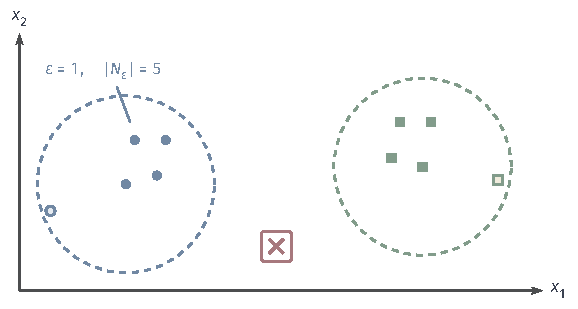
\includegraphics[width=97.850mm]{figures/04-classic-models/00-shared/tikz/clustering-dbscan/figure.pdf}
  \caption{DBSCAN的教学示意，取$\varepsilon=1$、$\mathrm{MinPts}=4$，计数包含自身。圆形和方形分别标识两个核心分量，颜色只作辅助；实心标记为核心点，浅色填充标记为边界点，红框叉号为噪声。虚线圆表示两个示例核心点的邻域；左侧标注直接给出邻域内计数，边界点不能继续扩展簇。}
 \label{fig:clustering-dbscan}
\end{figure}

\subsubsection{参数学习}

DBSCAN 的主要工作是查询邻域并搜索核心连通分量。代码~\ref{code:clustering-dbscan} 使用暴力距离查询，完整展示暂定噪声被重新吸收为边界点的情况。

\begin{codeblock}[language=Python,label={code:clustering-dbscan}]{DBSCAN 的邻域扩展}
import numpy as np
from collections import deque

def dbscan(X, eps, min_pts):
    X = np.asarray(X, dtype=float)
    if eps <= 0 or min_pts < 1:
        raise ValueError("invalid density parameters")
    labels = np.full(len(X), -1)  # -1 未访问，-2 噪声
    def neighbors(i):
        d2 = ((X - X[i]) ** 2).sum(1)
        return np.flatnonzero(d2 <= eps ** 2)
    cid = 0
    for i in range(len(X)):
        if labels[i] != -1:
            continue
        near = neighbors(i)
        if len(near) < min_pts:
            labels[i] = -2
            continue
        labels[i] = cid
        queue = deque(near)
        while queue:
            j = queue.popleft()
            if labels[j] == -2:
                labels[j] = cid
            if labels[j] != -1:
                continue
            labels[j] = cid
            near_j = neighbors(j)
            if len(near_j) >= min_pts:
                queue.extend(near_j)
        cid += 1
    return labels
\end{codeblock}

代码中每个样本至多查询一次邻域，队列则可能保存重复索引。暴力距离计算约需$O(n^2d)$运算。低维数据且邻域规模受控时，空间索引可使实践成本接近$O(n\log n)$；高维或大半径会增加访问量，最坏仍可达到平方级。预存全部邻域还可能占用$O(n^2)$内存。

参数选择可从第 $m$ 近邻距离的排序图入手，近邻计数约定应与是否包含自身一致。曲线的转折提示不同密度尺度，但未必存在清晰肘部。Schubert 等把 $\mathrm{MinPts}\approx 2d$ 作为平滑密度估计的经验起点，而不是一般最优值\scite{clust-schubert2017}。重复样本、噪声比例和有效维数都会影响合理的邻域大小与最小样本数。

\subsubsection{理论分析}

\paragraph{表达能力}
DBSCAN以核心点连通区域表达密度簇，可以保留非凸形状。一个共同邻域半径和阈值却未必能同时适应相差很大的密度，细桥或邻域尺度失配也会改变分组。

\paragraph{收敛性}
DBSCAN的访问和扩展在有限样本上结束，其计算任务是搜索核心连通分量。由于这里没有连续参数的迭代优化，需要验证的是搜索是否完整，以及固定数据下哪些输出与访问顺序无关。

\begin{theorem}[DBSCAN 的核心点确定性]
 \label{thm:clustering-dbscan}
 固定数据、对称相异度和参数 $(\varepsilon,m)$，DBSCAN 输出的每个簇限制到核心点后，恰为核心点邻接图的一个连通分量。因此核心点划分与访问顺序无关，簇编号的置换除外。
\end{theorem}
\begin{proof}
在核心点集合上，距离不超过 $\varepsilon$ 的两点能相互直接密度到达。有限链的连通关系满足自反、对称和传递性，故图的连通分量就是核心点上密度相连关系的等价类。

从任一尚未访问的核心点扩展时，每发现一个核心邻居就加入它的邻域。沿路径长度归纳，该点所在连通分量中的每个核心点最终都会被访问。反过来，扩展过程只能经由核心点邻接边到达其他核心点，不能穿过非核心边界点连接两个分量。因此输出的核心集合既不遗漏本分量，也不包含其他分量，结论成立。
\end{proof}

定理固定了核心点划分。一个边界点若邻接多个核心分量，其单一归属仍由访问规则决定；簇编号和共享边界归属是两种不同的顺序影响。

\paragraph{泛化性}
重新运行时，新增样本会改变邻域计数：原边界点可能达到核心阈值，新核心点也可能连接两个分量。因此，定理对固定数据的确定性与抽样扰动下的稳定性属于不同问题。

DBSCAN通常为当前样本给出分组。预测新样本时，可依据已有核心点的邻接关系定义分配，并规定多簇冲突和拒绝；将新样本纳入数据重新搜索则可能改变原分量。密度差异较大时，小$\varepsilon$可能拆开稀疏群组，大$\varepsilon$可能连上邻近稠密群组，尺度选择需同时检查这些影响。

\subsubsection{小结}

DBSCAN由局部计数产生核心点，再以连通性形成簇，并显式保留噪声。它省去预设$K$，同时引入全局半径、计数阈值及距离选择。可恢复的形状由密度连通定义决定，高维查询和不同密度群组仍可能限制实际效果。

\subsection{OPTICS}
\label{sec:clustering-optics}

反复调整 DBSCAN 的半径会重复查询相似邻域。OPTICS（Ordering Points To Identify the Clustering Structure）保留一次搜索中的密度排序，使分析者能够事后读取不同尺度的结构。Ankerst 等在 1999 年提出的方法输出排序与距离记录，而非直接输出唯一划分\scite{clust-ankerst1999}。

OPTICS把邻域计算与划分提取分开。DBSCAN在给定尺度后返回簇标签，OPTICS先保存访问次序和距离，供后续比较多种尺度。探索密度群组因而主要转为读取同一份结果，同时需要明确采用的提取规则。

\subsubsection{模型结构}

设搜索半径上限为 $\varepsilon_{\max}$。若样本 $i$ 在该半径内有至少 $m$ 个邻居，则其\term{核心距离}（core distance）为第 $m$ 近邻距离；否则记为 $+\infty$：
\[
 a_i=
 \begin{cases}
 \delta_{i,(m)},&|N_{\varepsilon_{\max}}(i)|\geq m,\\
 +\infty,&\text{其他情况}.
 \end{cases}
\]
由核心点 $i$ 到邻居 $j$ 的\term{可达距离}（reachability distance）定义为
\begin{equation}
 r(j\mid i)=\max\{a_i,\delta(\bm{x}_i,\bm{x}_j)\}.
 \label{eq:clustering-reachability}
\end{equation}
方向来自出发点的核心距离，因此通常 $r(j\mid i)\ne r(i\mid j)$。它表示在确保出发点足够密集的同时覆盖 $j$ 所需的半径。

OPTICS 为每个样本记录访问次序、核心距离和当前获得的最小可达距离。按访问次序画出可达距离形成\term{可达图}（reachability plot）；低谷通常对应容易从内部到达的密集区域，较高的过渡位置提示区域之间的分隔。

\subsubsection{参数学习}

从一个未处理点开始，算法输出该点并查询邻域。如果它是核心点，就用式~\eqref{eq:clustering-reachability} 更新未处理邻居的最小可达距离；优先队列每次取出当前可达距离最小的点，继续同样的过程。队列为空而仍有未处理点时，再开始一个新的搜索。这个过程是按可达距离优先的遍历，而不是普通先进先出的广度优先搜索。

给定 $\varepsilon'\leq\varepsilon_{\max}$，提取 DBSCAN 式结构时必须同时使用核心距离。沿排序扫描，若某点的记录可达距离大于 $\varepsilon'$，但核心距离不大于 $\varepsilon'$，它应开启一个新簇；若二者都大于阈值，才暂记为噪声；可达距离不大于阈值的点接续当前簇。只把水平线下的连续段当作簇，会漏掉可达距离很大、却负责开启新簇的核心点。不同提取规则对部分边界点的处理还可能与重新运行 DBSCAN 不同。

图~\ref{fig:clustering-optics-reachability} 将原始样本间距与可达图对应起来。中间一组样本较稀疏，形成的谷底较高；用 $\varepsilon'=0.35$ 提取时它们不构成核心簇，增大阈值才会纳入。次序 1、8、14 对应三次重新开始的搜索，其可达距离为无穷；次序 23 的孤立点也有无穷可达距离，但它的核心距离同样无穷，因而不能开启簇。

\begin{figure}[htbp]
  \centering
  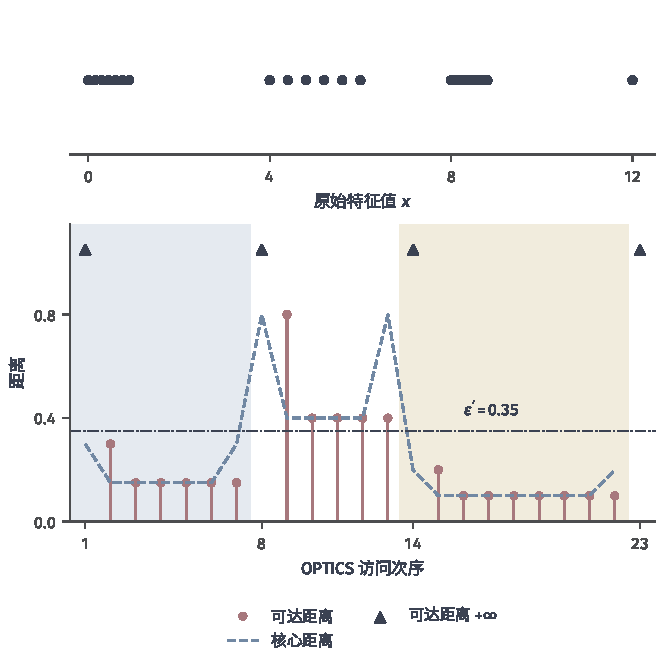
\includegraphics[width=105.412mm]{figures/04-classic-models/00-shared/matplotlib/clustering-optics-reachability/figure.pdf}
  \caption{固定一维教学数据上的OPTICS排序，取$\mathrm{MinPts}=3$（含自身）、$\varepsilon_{\max}=1.1$。三组样本的间距分别为$0.15$、$0.4$、$0.1$，另有$x=12$的孤立点。红色竖棒为可达距离，蓝色虚线为核心距离；蓝、黄底色标出两个低谷。无穷可达距离用顶部三角形表示，不能按其显示高度作数值比较；水平点划线展示阈值切割在本例中提取哪些低谷。}
 \label{fig:clustering-optics-reachability}
\end{figure}

低谷也可按相对陡降、陡升的$\xi$规则提取，并结合最小簇规模、前驱关系及嵌套处理。原始OPTICS已讨论陡峭区域，后续工作进一步构造密度层次。这里的自动提取减少人工读图，尺度和粒度仍由提取参数控制。

\subsubsection{小结}

OPTICS保留一次搜索中的多尺度结构，便于比较不同密度群组；结果受$\varepsilon_{\max}$、$\mathrm{MinPts}$和提取规则共同影响。空间索引与邻域规模有利时可减少搜索，最坏成本仍可能为平方级。优先队列和距离记录增加了操作与存储，应按同一数据和目标粒度与DBSCAN比较。

\subsection{Mean Shift}
\label{sec:clustering-mean-shift}

密度连通方法检查样本之间是否存在密集路径；\term{均值漂移}（Mean Shift）则在估计密度上搜索模态。它反复计算当前位置附近的加权均值并移动搜索点，先得到估计密度的驻点，再据起点的归宿形成分组。

% 两段历史含三条较长引文，同时为边栏预留空间。
\Needspace{125mm}
Fukunaga与Hostetler在1975年从密度梯度估计出发，将局部均值偏移用于模式识别\scite{clust-fukunaga1975}。搜索先回答密度增加的方向，再据轨迹确定归宿，因此无需预先给出簇边界。

Cheng在1995年推广核与权重，讨论均值漂移、模态搜索和聚类之间的联系\scite{clust-cheng1995}。Comaniciu与Meer在2002年系统分析该方法，并展示特征空间和图像分割中的应用\scite{clust-comaniciu2002}。这些工作将密度上的移动规则与随后得到的簇分配联系起来，二者仍需分别规定停止与合并方式。

\subsubsection{模型结构}

以径向核估计未知密度。设 $h>0$ 为带宽，核函数为 $\mathcal{K}(\bm{u})=c_k k(\lVert\bm{u}\rVert_2^2)$，其中$c_k$是归一化常数，$k$是剖面函数（profile），规定核权重怎样随距离平方变化。则\term{核密度估计}（kernel density estimation, KDE）为
\begin{equation}
 \hat f(\bm{y})=\frac{c_k}{nh^d}
 \sum_{i=1}^n
 k\left(\frac{\lVert\bm{y}-\bm{x}_i\rVert_2^2}{h^2}\right).
 \label{eq:clustering-kde}
\end{equation}
可以从各样本出发在估计密度上搜索，把趋向同一模态的起点归为一簇。带宽决定平滑尺度，小带宽通常保留细节，大带宽通常合并邻近结构；模态数量的具体变化还依赖维数、核与样本分布。

\subsubsection{参数学习}

令 $g(u)=-k'(u)$，并记 $u_i(\bm{y})=\lVert\bm{y}-\bm{x}_i\rVert_2^2/h^2$。直接对式~\eqref{eq:clustering-kde} 求导可得
\[
 \nabla\hat f(\bm{y})=
 \frac{2c_k}{nh^{d+2}}
 \sum_i g(u_i(\bm{y}))(\bm{x}_i-\bm{y}).
\]
只要权重和为正，梯度便是正系数乘以\term{均值漂移向量}
\[
 \bm{m}(\bm{y})=
 \frac{\sum_i g(u_i(\bm{y}))\bm{x}_i}
      {\sum_i g(u_i(\bm{y}))}-\bm{y}.
\]
因此采用下列自适应步长的梯度方向更新：
\begin{equation}
 \bm{y}^{(t+1)}=
 \frac{\sum_i w_i^{(t)}\bm{x}_i}{\sum_i w_i^{(t)}},
 \qquad w_i^{(t)}=g(u_i(\bm{y}^{(t)})).
 \label{eq:clustering-mean-shift}
\end{equation}
权重来自一元剖面函数的负导数$g$，其自变量是距离平方。高斯剖面$k(u)=\exp(-u/2)$给出与高斯权重成比例的$g$，Epanechnikov剖面$(1-u)_+$在支撑内部给出常数权重，边界按分段规则处理。

式~\eqref{eq:clustering-mean-shift}与第\ref{sec:regression-nadaraya-watson}节的Nadaraya--Watson回归都计算核加权平均。Mean Shift平均输入位置，更新搜索点；核回归平均响应，预测条件均值。相同的平均运算承担不同的估计任务。

图~\ref{fig:clustering-mean-shift-modes}固定同一组一维样本，两个起点沿式~\eqref{eq:clustering-mean-shift}分别向左右峰移动，靠近驻点时位移减小。灰线改用更大带宽，两个峰合为一个峰。起点决定从哪里搜索，带宽改变估计密度及可到达的模态，两项选择因而影响不同的对象。

\Needspace{90mm}
\begin{figure}[htbp]
  \centering
  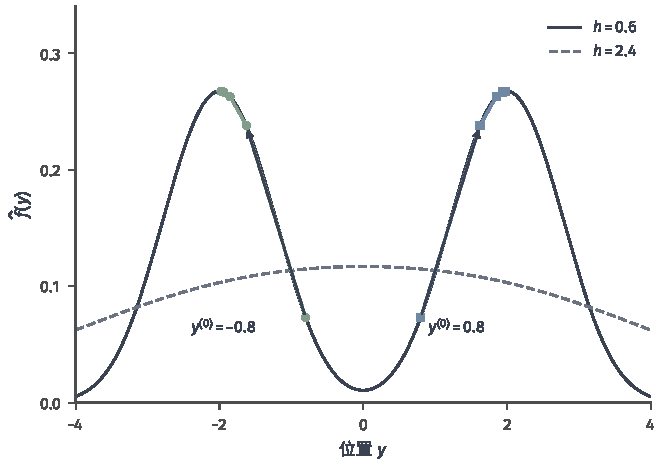
\includegraphics[width=105.412mm]{figures/04-classic-models/00-shared/matplotlib/clustering-mean-shift-modes/figure.pdf}
  \caption{Mean Shift 的密度爬升与带宽效应。左右各有三个样本，位置为 $-2.5,-2,-1.5$ 和 $1.5,2,2.5$，均采用高斯核。彩色标记给出带宽 $h=0.6$ 时从 $\pm0.8$ 出发的初始位置和四次更新，箭头指示第一次移动；灰色虚线对应 $h=2.4$，轨迹在黑色实线上计算。}
 \label{fig:clustering-mean-shift-modes}
\end{figure}

\begin{codeblock}[language=Python,label={code:clustering-mean-shift}]{高斯 Mean Shift 的起点更新}
import numpy as np

def mean_shift_positions(X, h, max_iter=300, tol=1e-4):
    X = np.asarray(X, dtype=float)
    if h <= 0:
        raise ValueError("h must be positive")
    Y = X.copy()
    for _ in range(max_iter):
        d2 = ((Y[:, None] - X[None]) ** 2).sum(2)
        log_w = -d2 / (2 * h * h)
        log_w -= log_w.max(1, keepdims=True)
        W = np.exp(log_w)
        new = (W @ X) / W.sum(1, keepdims=True)
        step = np.linalg.norm(new - Y, axis=1).max()
        Y = new
        if step <= tol:
            break
    return Y
\end{codeblock}

代码返回最终位置。得到簇标签还需合并相近终点，例如构造距离不超过$\rho$的终点图并取连通分量；$\rho=h/2$可作教学起点。这个合并阈值与更新容差用途不同，连通规则可能沿一串近终点把不同模态接在一起，需单独检查。

全部$n$个起点的一轮精确更新约需$O(n^2d)$运算。高斯核覆盖所有样本，因此截断邻域或近似近邻改变了精确更新。大数据实现可分块、减少起点或改用有限支撑核，并分别核对计算节省与位置误差。

\subsubsection{理论分析}

\paragraph{表达能力}
Mean Shift以核密度的吸引域组织簇，带宽决定哪些峰被保留。多个真实群体可能被平滑成一个峰，一个群体也可能对应多个峰；密度模态不必等同于任务类别。

\paragraph{收敛性}
Mean Shift的上升不等式控制密度值，位置收敛还需排除轨迹在多个聚点之间移动。步长平方可和只说明步长趋零，后续研究指出了将它直接推为Cauchy性的缺口\scite{clust-aliyari2015}。下面用紧性、连续性和有限固定点补足这一步。

\begin{theorem}[Mean Shift 的密度单调性与条件收敛]
 \label{thm:clustering-mean-shift}
 设 $k$ 非负、凸、非增且可微，$k(0)<\infty$，迭代中权重和始终为正。则式~\eqref{eq:clustering-mean-shift} 产生的密度值单调不减且收敛。若进一步假设 $g=-k'$ 连续且严格为正，样本凸包内的固定点只有有限个，则位置序列也收敛，极限为 $\hat f$ 的驻点。
\end{theorem}
\begin{proof}
简记 $\bm{y}=\bm{y}^{(t)}$、$\bm{y}'=\bm{y}^{(t+1)}$。由凸性，
\[
 k(u_i(\bm{y}'))-k(u_i(\bm{y}))
 \geq g(u_i(\bm{y}))
       \bigl(u_i(\bm{y})-u_i(\bm{y}')\bigr).
\]
令 $w_i=g(u_i(\bm{y}))$、$s=\sum_iw_i$。由于 $\bm{y}'$ 是加权均值，展开平方后交叉项为零，得到
\[
 \sum_iw_i\bigl(
 \lVert\bm{y}-\bm{x}_i\rVert_2^2
 -\lVert\bm{y}'-\bm{x}_i\rVert_2^2\bigr)
 =s\lVert\bm{y}'-\bm{y}\rVert_2^2.
\]
所以
\begin{equation}
 \hat f(\bm{y}')-\hat f(\bm{y})
 \geq\frac{c_k s}{nh^{d+2}}
       \lVert\bm{y}'-\bm{y}\rVert_2^2\geq0.
 \label{eq:clustering-mean-shift-ascent}
\end{equation}
又有 $\hat f(\bm{y})\leq c_k k(0)/h^d$，故密度值收敛。

在附加条件下，第一次更新后所有位置均在有限样本的紧凸包内。距离平方因此有界，而连续正函数 $g$ 在相应紧区间上有正下界，故 $s$ 也有统一正下界。对式~\eqref{eq:clustering-mean-shift-ascent} 求和，得到步长平方可和，特别地，$\lVert\bm{y}^{(t+1)}-\bm{y}^{(t)}\rVert_2\to0$。

记连续更新映射为 $T$。任取收敛子列 $\bm{y}^{(t_j)}\to\bm{y}^\ast$，步长趋零与连续性给出 $T(\bm{y}^\ast)=\bm{y}^\ast$，所以每个聚点都是固定点。固定点有限，取彼此不相交的小球包围它们；序列最终必在这些小球的并集中，否则紧性会产生球外聚点。步长最终小于球之间的间隙，故序列不能再从一个球跳到另一个球。任意缩小球半径，便知它只能趋向其中一个固定点。梯度公式最后给出 $\nabla\hat f(\bm{y}^\ast)=\bm{0}$。
\end{proof}

位置收敛由紧性、连续性及有限固定点共同支持，平方可和用于先证明步长趋零。极限是驻点，特殊起点可能停在鞍点；解释为密度峰还需检查局部形状。Epanechnikov核的分段边界和零权重不满足第二部分的全部条件，需另作分析。

\paragraph{泛化性}
留出样本上的模态结构取决于带宽及密度估计误差。KDE在适当光滑性和随$n$缩小的带宽等条件下可一致估计密度；从密度误差控制到峰位置、吸引域和簇分配的稳定，还需正则条件。当前固定KDE上的上升定理只处理搜索计算。

\subsubsection{小结}

Mean Shift以局部加权均值实现密度爬升，随后按模态归宿组织簇。簇数由带宽、起点和终点合并共同决定。图像分割与跟踪可利用这种聚集机制，使用时需同时检查计算预算、驻点类型及带宽变化下的分组。

\subsection{模型对比与总结}

三种邻域方法形成不同输出：DBSCAN给固定尺度下的核心连通簇，OPTICS保存多尺度排序，Mean Shift搜索平滑密度的驻点。连通区域含多个峰时，结果可在相近尺度下不同。噪声拒绝也需逐方法检查；下面的扩展进一步把网格或层次加入密度表示。

DENCLUE叠加样本影响函数形成密度，用吸引点及其连通关系组织簇，以密度阈值标记噪声，并借网格辅助计算\scite{clust-hinneburg1998}。它与Mean Shift共享密度估计视角，估计在高维是否可靠仍取决于样本量、表示和核尺度。

HDBSCAN 把核心距离用于定义\term{互可达距离}（mutual reachability distance）：
\[
 \delta_{\mathrm{mr}}(i,j)
 =\max\{a_i,a_j,\delta(\bm{x}_i,\bm{x}_j)\}.
\]
在这一距离上构造最小生成树并形成密度层次，再按最小簇规模压缩层次、按跨尺度持续性选择簇，可以减轻单一 $\varepsilon$ 的限制。Campello 等给出了这一层次密度框架\scite{clust-campello2013}。

HDBSCAN的跨尺度持续性是层次中的簇选择量，评估抽样扰动还需要另外的统计协议。最小簇规模等参数继续控制输出，高维距离的区分度也需检验。密度路线将低密度分隔纳入簇定义；已有可信样本关系时，还可直接用图建立群组。

\section{基于图的聚类}
\label{sec:clustering-graph}

社交连接、文档相似度和像素邻接可以直接表示为加权图。图聚类将样本作为顶点、相似程度作为边权，寻找内部连接较强而外部连接较弱的群组。向量距离也可用于建图；边权和邻域规则因此继续决定所保留的相似关系。

仅最小化切边权重，可能轻易切下一个连接少的小块。对簇规模或连接体积作归一化，可以比较“割断多少联系”与“簇原来拥有多少联系”。谱聚类再把这一离散搜索松弛为特征向量求解。

\subsection{谱聚类}
\label{sec:clustering-spectral}

\term{谱聚类}（spectral clustering）先以图拉普拉斯的特征向量表示顶点，再将顶点划分为簇。第\ref{sec:dim-le}节的拉普拉斯特征映射共享建图与低频谱表示，但输出连续坐标；聚类还需要离散分配。von Luxburg的教程整理了图构造、归一化及适用条件\scite{clust-luxburg2007}。下面以归一化割及多簇谱算法展开这一流程。

Donath与Hoffman在1973年用谱信息给图划分代价建立下界，将组合搜索与可计算特征值联系起来\scite{clust-donath1973}。Shi与Malik进一步用像素相似关系建立归一化割，相关会议和期刊论文分别发表于1997年和2000年\scite{clust-shi2000}。Ng、Jordan与Weiss在2001年会议提出多簇谱嵌入与行归一化，论文集于2002年出版\scite{clust-ng2002}。这些工作分别解释了图目标、连续表示及离散化的连接。

\subsubsection{模型结构}

设无向图的非负对称权重矩阵为 $\bm{W}\in\mathbb{R}^{n\times n}$，通常令 $w_{i,i}=0$。向量样本可用高斯相似度 $\exp(-\lVert\bm{x}_i-\bm{x}_j\rVert_2^2/(2\sigma^2))$ 构造边；近邻图则保留部分局部关系。单向近邻关系未必对称，必须明确采用并集对称化还是互近邻规则。

定义顶点度 $d_i=\sum_jw_{i,j}$、度矩阵 $\bm{D}=\operatorname{diag}(d_1,\ldots,d_n)$，以及三种拉普拉斯：
\begin{align}
 \bm{L}&=\bm{D}-\bm{W},\nonumber\\
 \bm{L}_{\mathrm{sym}}
 &=\bm{I}-\bm{D}^{-1/2}\bm{W}\bm{D}^{-1/2},\nonumber\\
 \bm{L}_{\mathrm{rw}}
 &=\bm{I}-\bm{D}^{-1}\bm{W}.
 \label{eq:clustering-laplacians}
\end{align}
归一化所用逆度数要求$d_i>0$，因此先单独处理孤立顶点。$\bm{L}_{\mathrm{rw}}$ 一般不对称，但与 $\bm{L}_{\mathrm{sym}}$ 相似，因而有相同的实特征值。对任意 $\bm{v}\in\mathbb{R}^n$，
\begin{equation}
 \bm{v}^{\top}\bm{L}\bm{v}
 =\frac12\sum_{i,j}w_{i,j}(v_i-v_j)^2\geq0.
 \label{eq:clustering-laplacian-form}
\end{equation}
所以 $\bm{L}$ 半正定，且 $\bm{L}\bm{1}=\bm{0}$；零特征值的重数等于连通分量数，图连通时才为单重。

归一化还具有随机游走解释。转移矩阵 $\bm{P}=\bm{D}^{-1}\bm{W}$ 让游走者按边权比例选择下一顶点，且 $\bm{L}_{\mathrm{rw}}=\bm{I}-\bm{P}$。从一个簇出发，若内部连接强而外部连接弱，游走就倾向在簇中停留较久；Meilă 与 Shi 据此研究了聚类的随机游走视角\scite{clust-meila2001}。

设 $\operatorname{cut}(A,\bar A)=\sum_{i\in A,j\notin A}w_{i,j}$，$\operatorname{vol}(A)=\sum_{i\in A}d_i$。\term{归一化割}（normalized cut, NCut）定义为
\begin{equation}
 \operatorname{NCut}(\mathcal{P})
 =\sum_{k=1}^K
 \frac{\operatorname{cut}(C_k,\bar C_k)}
      {\operatorname{vol}(C_k)}.
 \label{eq:clustering-ncut}
\end{equation}
它比较切边与簇内外连接体积，减轻小簇的偏好；同体积的簇可以含不同样本数\scite{clust-shi2000}。\term{比率割}（RatioCut）则把分母换成 $|C_k|$，对应未归一化拉普拉斯的松弛。

\subsubsection{参数学习}

为把 NCut 改写成矩阵目标，定义 $\bm{F}\in\mathbb{R}^{n\times K}$，其中
\[
 f_{i,k}=
 \begin{cases}
  1/\sqrt{\operatorname{vol}(C_k)},&i\in C_k,\\
  0,&i\notin C_k.
 \end{cases}
\]
簇互不相交给出 $\bm{F}^{\top}\bm{D}\bm{F}=\bm{I}_K$。由式~\eqref{eq:clustering-laplacian-form}，第 $k$ 列的二次型恰为第 $k$ 项归一化割，故目标为 $\operatorname{tr}(\bm{F}^{\top}\bm{L}\bm{F})$。

困难在于每行只允许一个特定的非零值。去掉这一离散约束，令 $\bm{H}=\bm{D}^{1/2}\bm{F}$，得到
\begin{equation}
 \min_{\bm{H}^{\top}\bm{H}=\bm{I}_K}
 \operatorname{tr}(\bm{H}^{\top}
                   \bm{L}_{\mathrm{sym}}\bm{H}).
 \label{eq:clustering-spectral-relaxation}
\end{equation}
Shi--Malik 方法也可写为广义特征问题 $\bm{L}\bm{f}=\lambda\bm{D}\bm{f}$，与归一化变换相联系\scite{clust-shi2000}。取 $\bm{L}_{\mathrm{sym}}$ 最小的 $K$ 个特征值对应的特征向量，即得到式~\eqref{eq:clustering-spectral-relaxation} 的最优解；下文说明这一连续最优值及其唯一性条件。

连续解还需离散化。\term{NJW 算法}把 $\bm{H}$ 每一行归一化到单位长度，再对行向量运行 K-means\scite{clust-ng2002}。若图恰有 $K$ 个连通分量，理想谱空间中每个分量对应同一方向；行归一化消除度数造成的长度差异，图~\ref{fig:clustering-spectral} 展示了这一解释。连接较弱的实际图中，这只是近似结构。

\Needspace{62mm}
\begin{figure}[htbp]
  \centering
  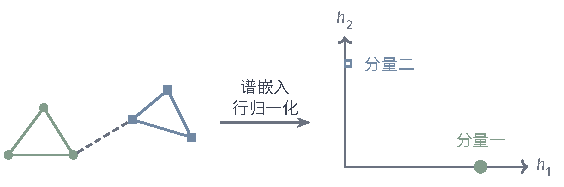
\includegraphics[width=95.564mm]{figures/04-classic-models/00-shared/tikz/clustering-spectral/figure.pdf}
  \caption{谱聚类的理想情形：圆形与方形分别标识两个互不连接的分量，颜色只作辅助；在归一化谱空间中，两个分量分别落到两个方向。细虚线表示实际数据中可能存在的弱连接；加入这些连接后，谱坐标通常形成近似群组。}
 \label{fig:clustering-spectral}
\end{figure}

\begin{codeblock}[language=Python,label={code:clustering-spectral}]{给定相似度矩阵的 NJW 算法}
import numpy as np
from scipy.linalg import eigh

def spectral_clustering(W, K):
    W = np.asarray(W, dtype=float)
    n = len(W)
    if W.shape != (n, n) or not 1 <= K <= n:
        raise ValueError("invalid shape or K")
    if (W < 0).any() or not np.allclose(W, W.T):
        raise ValueError("W must be nonnegative and symmetric")
    degree = W.sum(1)
    if (degree <= 0).any():
        raise ValueError("handle isolated vertices first")
    inv = 1 / np.sqrt(degree)
    L = np.eye(n) - inv[:, None] * W * inv[None, :]
    _, H = eigh(L, subset_by_index=[0, K - 1])
    length = np.linalg.norm(H, axis=1)
    if (length == 0).any():
        raise ValueError("zero embedding row")
    labels, _ = kmeans(H / length[:, None], K)
    return labels
\end{codeblock}

代码复用代码~\ref{code:clustering-kmeans}的K-means函数，处理能放入内存的稠密矩阵。图的连通分量数超过$K$时，所选零特征子空间可能含零行，也可能将多个分量任意合并。应先确定各连通分量是否需要独立输出，再选择谱子空间与分配策略。

稠密建图约需$O(n^2d)$距离运算和$O(n^2)$存储，完整特征分解约需$O(n^3)$。只求部分特征向量时，可用Lanczos或LOBPCG，矩阵乘法成本可按稀疏边数计算；迭代总成本还受特征间隙、精度和迭代次数影响。大规模实现可结合近邻图或Nyström近似，并核对它们对谱表示的误差。

\subsubsection{理论分析}

\paragraph{表达能力}
谱聚类用相似图的低频子空间表达分组，能够利用非凸连接结构。相似度、邻域构造与簇数决定候选划分；错误连接可能在谱求解之前已混合所需结构。

\paragraph{收敛性}
谱聚类的求解分为特征子空间计算与离散分组。前一阶段要找到最小的$K$个特征值及其子空间，并达到残差精度；后一阶段的K-means另有初始化与停止条件。下面先确定连续松弛的全局最优值，随后再说明它与离散图割质量的关系。

在式~\eqref{eq:clustering-spectral-relaxation}中，令$\bm B=\bm L_{\mathrm{sym}}$，并取$1\leq K\leq n$。将这个实对称谱算子的特征值按升序记为$\lambda_1\leq\cdots\leq\lambda_n$，对应标准正交特征向量为$\bm u_1,\ldots,\bm u_n$。正交列约束下的连续松弛最优值为
\[
 \min_{\bm H^\top\bm H=\bm I_K}
 \operatorname{tr}(\bm H^\top\bm B\bm H)
 =\sum_{k=1}^K\lambda_k.
\]
取$\bm H=[\bm u_1,\ldots,\bm u_K]$即可达到该值。若$K<n$且$\lambda_K<\lambda_{K+1}$，最优列空间唯一，但其中的正交基仍可右乘正交矩阵（参考\BookTheoremRef{thm:matrix-analysis-trace-minimum}{第一卷“数学准备”的“正交列约束下的迹最小化”定理}）。这个结论确定的是连续子空间；把它转换成离散簇标签，还需要前述离散化步骤。

图割质量与谱量之间还存在 Cheeger 型联系。对连通、非负无向图，定义\term{电导}（conductance）
\[
 \phi(S)=
 \frac{\operatorname{cut}(S,\bar S)}
 {\min\{\operatorname{vol}(S),\operatorname{vol}(\bar S)\}},
 \qquad h_G=\min_{\varnothing\ne S\ne V}\phi(S).
\]
若 $\lambda_2$ 是 $\bm{L}_{\mathrm{sym}}$ 的第二小特征值，则
\begin{equation}
 \frac{\lambda_2}{2}\leq h_G\leq\sqrt{2\lambda_2}.
 \label{eq:clustering-cheeger}
\end{equation}
图上的这类不等式把低频特征向量与稀疏切割联系起来，标准谱图论教材给出了证明及其与流形版本的关系\scite{clust-chung1997}。

这里$h_G$最小化电导，NCut则对两个方向分别按体积归一；二者的关系需由分母比较得到。二分情形满足 $\phi(S)\leq\operatorname{NCut}(S,\bar S)\leq2\phi(S)$。若 $\bm{u}$ 是 $\bm{L}_{\mathrm{sym}}$ 的第二特征向量，则
\[
 \bm{f}=\bm{D}^{-1/2}\bm{u},
 \qquad
 \bm{L}\bm{f}=\lambda_2\bm{D}\bm{f},
 \qquad
 \bm{L}_{\mathrm{rw}}\bm{f}=\lambda_2\bm{f}.
\]
因此，Cheeger sweep 应按 $f_i=u_i/\sqrt{d_i}$ 排序并扫描阈值；若直接求广义特征问题或随机游走拉普拉斯，排序坐标就是其特征向量 $\bm{f}$。只有各顶点度数相同时，按 $\bm{u}$ 与按 $\bm{f}$ 排序才必然相同。这一保证对应二分的阈值扫描；多簇NJW加K-means使用另一离散化规则，其图割质量需另行分析。

\paragraph{泛化性}
经验谱对象还需与总体分布联系。von Luxburg、Belkin与Bousquet研究了固定相似核下，经验谱对象向总体积分算子的收敛\scite{clust-luxburg2008}。核、度函数及谱隔离条件控制这种极限，归一化与未归一化方法的前提不同；从谱收敛到簇分配，还需检查离散化的稳定性。

带宽随样本量改变时，可以进一步研究流形上的拉普拉斯--贝尔特拉米极限。此时需规定带宽变化、流形光滑性、采样密度和归一化方式，与固定核的总体积分算子属于不同设定。统计结论应按相应的建图制度使用。

\subsubsection{小结}

谱聚类以关系图保留非凸连接结构，用特征分解求连续松弛，再通过离散化形成簇。图构造与最后分配共同影响结果。特征值间隙可作为探索$K$的线索，解释时还需排查噪声、弱连接与孤立分量造成的间隙。

\subsection{模型对比与总结}

谱聚类先建图，再松弛图割并离散化。其他图方法可以改为搜索典型代表或社区；下面比较它们使用的消息和目标。\term{近邻传播}（Affinity Propagation, AP）把每个样本作为潜在代表，以适合度和可用度两类消息协调代表选择。给定相似度 $s(i,k)$，其典型更新为
\[
 r(i,k)=s(i,k)-\max_{k'\ne k}\{a(i,k')+s(i,k')\},
\]
\[
 a(i,k)=
 \min\left\{0,r(k,k)+
 \sum_{i'\notin\{i,k\}}\max\{0,r(i',k)\}\right\},
 \quad i\ne k,
\]
而 $a(k,k)=\sum_{i'\ne k}\max\{0,r(i',k)\}$。适合度衡量候选相对其他代表的优势，可用度汇总其他样本对该代表的支持。对角相似度 $s(k,k)$ 是偏好参数，间接控制代表数；通常还需阻尼以缓解振荡，迭代不保证总收敛\scite{clust-frey2007}。

消息更新后，以两类消息之和比较候选代表，并按预定平局规则选择代表索引
\[
 e_i\in\argmax_k\{a(i,k)+r(i,k)\}.
\]
同一代表对应同一簇，即$C_k=\{i:e_i=k\}$。输出要求代表选择连续若干轮稳定且相互一致：一个样本选择$k$时，$e_k=k$，即代表选自身。中间迭代可能尚未满足这两个条件，此时继续更新或返回未收敛状态，保留当前消息供诊断。

社区发现中的 Louvain 方法则优化\term{模块度}（modularity），比较实际簇内边权与保留度数的随机基准。令 $2m_G=\sum_i d_i$，典型目标为
\[
 Q=\frac{1}{2m_G}\sum_{i,j}
 \left(w_{i,j}-\frac{d_i d_j}{2m_G}\right)
 \mathbb{1}\{c_i=c_j\}.
\]
局部顶点移动提高模块度，社区凝聚再改变搜索规模，稀疏图可减少边访问。结果仍受分辨率、移动顺序和局部极值影响；其目标与NCut不同，保证应按模块度搜索核对\scite{clust-blondel2008}。

谱聚类、AP和Louvain都以关系为输入，目标分别侧重切割、代表支持和相对随机基准的社区边权。选择时应先规定希望输出低电导集合、典型代表还是高模块度社区，再据同一任务评价计算与分组质量。

\section{基于网格与子空间的聚类}
\label{sec:clustering-subspace}

大样本的点对访问可能超过预算，无关特征也可能掩盖只在少数坐标上聚集的群组。一些高维分布会使最近与最远距离的相对差异减小；是否发生这种集中，仍取决于数据结构与表示。网格和子空间方法分别处理重复访问与相关坐标选择。

网格方法把样本汇为单元统计，减少随后查询原始点的次数。子空间方法寻找群组在哪些坐标上紧凑，并允许各簇使用不同特征。CLIQUE结合两者，以计数剪枝降低候选搜索；已存单元和子空间组合也可能随维数快速增长，需要计入资源预算。

\subsection{STING}

若需要反复查询“哪些区域足够密集”，可以预先保存区域统计。\term{统计信息网格}（STatistical INformation Grid, STING）由 Wang、Yang 与 Muntz 在 1997 年提出，用层次网格组织空间数据，查询时优先读取摘要\scite{clust-wang1997}。

\subsubsection{模型结构}

STING通常用于低维空间的矩形层次网格。二维单元可分为四个子单元，$d$维完整二分则产生$2^d$个子单元。实现可只保存有记录或需要查询的单元，以控制空单元的存储。

单元摘要包含计数、各维均值、标准差、极值与分布类型估计。计数、和及平方和可由子单元相加，得到父单元的矩统计。分布类型则属于近似描述：子单元合并后形成混合，父单元可能超出原分布族。

\subsubsection{参数学习}

构建阶段扫描样本，确定最细单元并更新统计，再自底向上汇总。固定维数和网格规模时可按 $O(n)$ 扫描成本理解；更完整地计入维数与 $G$ 个已存单元，代价包含 $O(nd+Gd)$，还取决于定位单元的数据结构。

查询时，从某层网格出发，依据摘要估计单元满足条件的可能性。例如，对密度条件使用计数，对属性范围条件使用极值或分布近似；排除不相关单元，对保留单元继续下钻。最终可以把满足密度条件且相邻的单元连成区域，必要时回到原始样本作精确检查。

固定摘要上的单元访问约按$O(G)$计，初始读入与统计仍需前述样本扫描。精确查询若最终检查$n_{\mathrm{scan}}$条原始记录，也应另外计费。基于估计概率的排除可能漏检；需要完整结果时，筛选规则须能证明被排除区域无法满足查询。

\subsubsection{小结}

STING以一次预处理建立可重复使用的区域摘要，适合低维查询和增量统计。边界精度由网格分辨率决定，倾斜结构可能横跨多个轴对齐单元。深度$L$的完整二分网格可有$2^{Ld}$个最细单元，高维应用需控制存储与细分范围。

\subsection{CLIQUE}
\label{sec:clustering-clique}

一组客户可能在购买频次和品类上集中，在年龄上却分散。寻找这种群组需要选择相关坐标，而非要求全维距离都小。Agrawal等在1998年提出CLIQUE（CLustering In QUEst），主动搜索含密集网格单元的坐标子空间\scite{clust-agrawal1998}。

STING与CLIQUE都将数据组织纳入数据库中的聚类计算。STING预存空间统计，节省重复查询；CLIQUE借用频繁模式的逐层筛选，节省高维组合检查。两者减少的是不同操作，可按查询频率与候选规模分别评价。

\subsubsection{模型结构}

每维划分为 $\xi$ 个区间，区间边界采用统一的半开约定，并把最后端点纳入最后一区间。对特征索引集合 $S\subseteq\{1,\ldots,d\}$，一个单元 $U$ 是所选坐标上区间的笛卡尔积。定义支持计数
\[
 n(U)=|\{i:\bm{x}_{i,S}\in U\}|.
\]
若 $n(U)\geq\tau$，则称 $U$ 为\term{密集单元}（dense unit）。跨维沿用同一计数阈值$\tau$，固定样本比例阈值在样本数相同时等价。按单元体积定义的密度改变了跨维比较尺度，需另设阈值与剪枝条件。

同一子空间内，两个单元若仅沿一个坐标方向相邻而其他区间相同，就视为邻接；密集单元的极大连通分量构成簇。输出是“子空间与簇”的集合，同一样本可以在不同子空间出现于多个簇，也可以未被任何簇覆盖。图~\ref{fig:clustering-subspace} 表示高维单元投影后样本计数只会增加的关键性质。

\begin{figure}[htbp]
  \centering
  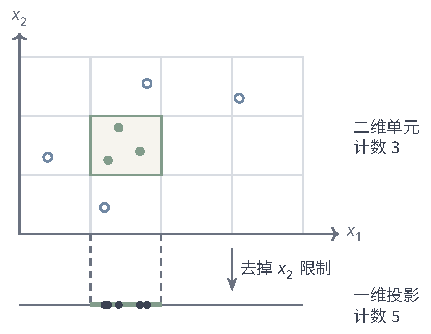
\includegraphics[width=72.912mm]{figures/04-classic-models/00-shared/tikz/clustering-subspace/figure.pdf}
  \caption{CLIQUE 的投影计数示意。二维高亮单元含三个样本，其在横轴区间上的投影还包含其他纵坐标范围的样本。取共同阈值 $\tau=3$，二维单元密集必然推出对应一维单元密集，反方向则不成立。}
 \label{fig:clustering-subspace}
\end{figure}

\subsubsection{参数学习}

CLIQUE 借鉴 Apriori 的逐层候选生成。扫描数据找到一维密集单元后，把具有兼容低维区间的单元连接成更高维候选；只有所有低一维投影都密集的候选才继续计数验证。重复直到候选为空或达到搜索维数上限。

在保留下来的子空间中，算法连接相邻密集单元，形成簇，并可用轴对齐区域的析取式压缩簇描述。原始方法还包含选择子空间和简化描述的步骤；若使用额外启发式筛选，完整性应相对于筛选后的搜索范围表述。

\subsubsection{理论分析}

\paragraph{表达能力}
CLIQUE用轴对齐网格中的密集单元及其连通性表示子空间簇。网格与坐标选择限制边界精度，斜向或跨格稀释的结构可能需要更细网格和更高搜索成本。

\paragraph{收敛性}
CLIQUE 每轮增加候选的维数，最多搜索到 $d$ 维，因此在有限网格上必然结束。除了终止性，还需证明提前剪枝不会遗漏满足计数条件的高维单元；下面的向下封闭性给出这一保证。

\begin{theorem}[子空间密集性的向下封闭性]
 \label{thm:clustering-clique}
 在一致的逐维网格和共同计数阈值 $\tau$ 下，若 $S$ 上的单元 $U$ 密集，则对任意非空 $S'\subseteq S$，其投影 $U|_{S'}$ 也密集。
\end{theorem}
\begin{proof}
记 $I(U)=\{i:\bm{x}_{i,S}\in U\}$。若 $i\in I(U)$，它在 $S$ 的所有选定坐标上都满足区间限制，去掉部分坐标限制后仍然满足。因此
\[
 I(U)\subseteq I(U|_{S'}),\qquad
 n(U|_{S'})\geq n(U)\geq\tau.
\]
投影网格沿用相同区间，故 $U|_{S'}$ 是合法低维单元，并达到同一密集阈值。
\end{proof}

向下封闭性允许根据不密集的低维投影排除高维候选。多个投影各自密集时，其中的样本可能不同，所以高维计数仍需验证。该论证使用共同计数阈值；改为按体积归一的密度或随维数变化的阈值时，需重新核对剪枝条件。

有限网格保证搜索最终结束，但最坏情况下大量投影都密集，仍可能枚举指数多个子空间和单元。

\paragraph{泛化性}
样本中的密集单元能否代表总体群组，取决于抽样、网格和阈值。阈值附近的单元可能因少量样本改变而由密变稀，进而拆开或连接整个网格簇。验证时可重采样并平移网格，检查区域计数与连通结构；这项统计检验与候选剪枝的搜索完整性分工不同。

\subsubsection{小结}

CLIQUE为各簇保留相关坐标，并以向下封闭性减少无效候选。粗网格可能混合相邻群体，细网格可能稀释计数，轴对齐则限制可表达的子空间方向。MAFIA、SUBCLU与DOC/FASTDOC分别调整网格、密度连通和搜索，以处理这些限制。

\subsection{模型对比与总结}

STING建立可重复查询的空间摘要，CLIQUE发现不同坐标上的群组；两者分别节省原始样本访问与全维结构要求。可扩展性仍由摘要单元和候选规模限制。下面沿多分辨率、密度子空间和投影搜索三个方向继续比较。

WaveCluster把网格计数作为离散信号，在不同小波尺度寻找密集区域，并抑制部分高频噪声\scite{clust-sheikholeslami1998}。分辨率继续限定边界精度。固定维数、网格及变换规模时，读入成本可随样本数线性增长，网格变换和区域提取仍需单独计入。

SUBCLU在子空间中采用DBSCAN的密度连通，减少固定网格边界的影响；MAFIA用自适应区间调整候选，DOC与FASTDOC用随机抽样找投影中的紧凑群组\scite{clust-parsons2004}。各方法的邻域、阈值和候选条件不同，搜索保证需由对应定义建立。

\term{投影聚类}（projected clustering）通常要求每个样本有唯一簇归属，同时为每簇寻找相关子空间。PROCLUS 使用类似 K-medoids 的代表搜索并选择相关坐标；ORCLUS 进一步学习任意方向的低维正交投影，能够表达相对坐标轴倾斜的群组。前者偏向坐标子集，后者需估计方向，两者的计算与统计代价因此不同。

需要多个重叠解释时，可评价CLIQUE或SUBCLU；要求唯一簇归属及每簇相关坐标时，可评价投影方法。选择前还需核对数据是否存在所假设的低维集中结构，搜索算法只能从已有信息中恢复它。

\section{基于层次的聚类}
\label{sec:clustering-hierarchy}

探索阶段的群组粒度尚不明确时，可以保留多个层级。\term{层次聚类}（hierarchical clustering）用\term{树状图}（dendrogram）记录嵌套的合并或分裂，使分析者从同一棵树读取不同规模的划分。具体截取哪一层，仍由任务用途与证据确定。

凝聚方法从单点向上合并，分裂方法从全集向下拆分。图~\ref{fig:clustering-dendrogram}在同一棵树上读取两种粒度；截线保留已完成的层次决策，不对该粒度重新搜索。

\begin{figure}[htbp]
  \centering
  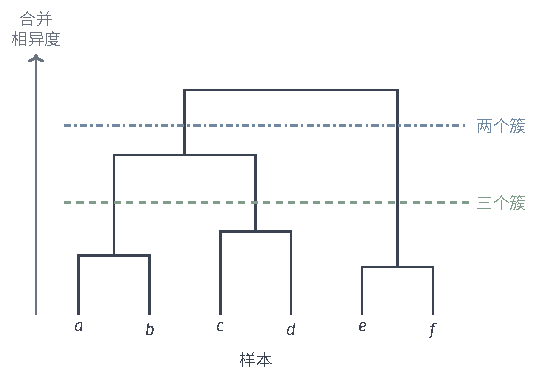
\includegraphics[width=90.914mm]{figures/04-classic-models/00-shared/tikz/clustering-dendrogram/figure.pdf}
  \caption{教学用层次树。叶节点为六个样本，内部节点高度表示合并相异度。较低截线得到三个簇，较高截线得到两个簇；图中高度为示意数值。}
 \label{fig:clustering-dendrogram}
\end{figure}

\subsection{AGNES（凝聚层次聚类）}
\label{sec:clustering-agnes}

\term{凝聚分析}（Agglomerative Nesting, AGNES）每次合并当前相异度最小的两簇。Kaufman与Rousseeuw在1990年的专著中将这一长期用于数值分类学的过程与自顶向下的DIANA并列介绍。其主要设计问题是簇间相异度如何从样本关系计算。

链接准则把不同群组偏好写进合并决策：单链接沿最近联系扩展，平均链接综合跨簇距离，Ward在1963年以最小SSE增量选择合并。凝聚方向规定构造顺序，链接准则决定哪种关系先进入树。

\subsubsection{模型结构}

初始划分为 $\mathcal{P}^{(0)}=\{\{1\},\ldots,\{n\}\}$。第 $t$ 步选择使 $D(A,B)$ 最小的两个当前簇，替换为 $A\cup B$，经过 $n-1$ 次合并得到根节点。固定相异度和确定的平局规则后，整棵树随之确定。

不同\term{链接方式}（linkage）用不同的簇间统计量：
\begin{align*}
 D_{\mathrm{single}}(A,B)
   &=\min_{i\in A,j\in B}\delta(\bm{x}_i,\bm{x}_j),\\
 D_{\mathrm{complete}}(A,B)
   &=\max_{i\in A,j\in B}\delta(\bm{x}_i,\bm{x}_j),\\
 D_{\mathrm{average}}(A,B)
   &=\frac{\sum_{i\in A,j\in B}\delta(\bm{x}_i,\bm{x}_j)}
   {|A||B|}.
\end{align*}
单链接沿近邻链扩展，可以保留细长形状，也容易被稀疏桥接点连接起来；全链接控制跨簇最远距离，倾向紧凑群组；平均链接考虑所有跨簇样本对，减弱单个极值的影响。这里的平均链接指按样本数加权的 UPGMA。

若样本处于欧氏空间，Ward 链接以合并引起的 SSE 增量定义相异度：
\[
 D_{\mathrm{Ward}}(A,B)
 =\mathrm{SSE}(A\cup B)-\mathrm{SSE}(A)-\mathrm{SSE}(B).
\]
它与 K-means 共享平方误差准则，但只允许合并已有簇。Ward 的原始工作明确以这种误差增量组织层次\scite{ward1963}。

\subsubsection{参数学习}

实现 AGNES 时，可以维护当前簇间的相异度，并在每次合并后更新相关行列。算法~\ref{alg:clustering-agnes} 省去了不影响定义的矩阵下标管理。

\begin{algorithm}[凝聚层次聚类]
 \label{alg:clustering-agnes}
 \begin{algorithmic}[1]
 \Require 样本相异度、链接方式和确定的平局规则
 \Ensure 包含合并高度的层次树
 \State 建立 $n$ 个单点簇，初始化簇间相异度
 \While{当前簇数大于 $1$}
  \State 选择使 $D(A,B)$ 最小的当前簇对
  \State 记录子簇 $A,B$ 和合并高度 $D(A,B)$
  \State 用 $A\cup B$ 替换 $A,B$
  \State 更新新簇与其他当前簇的相异度
 \EndWhile
 \end{algorithmic}
\end{algorithm}

Lance--Williams 递推使多种链接共享更新形式\scite{clust-lance1967}。
\begin{equation}
 \begin{aligned}
 D(A\cup B,C)={}&\alpha_A D(A,C)+\alpha_B D(B,C)\\
 &+\beta D(A,B)
 +\gamma|D(A,C)-D(B,C)|.
 \end{aligned}
 \label{eq:clustering-lance-williams}
\end{equation}
单链接的系数为 $(1/2,1/2,0,-1/2)$，全链接为 $(1/2,1/2,0,1/2)$，平均链接为 $(|A|/(|A|+|B|),|B|/(|A|+|B|),0,0)$。若 $D$ 直接表示 Ward 的 SSE 增量，令 $s=|A|+|B|+|C|$，则
\[
 \alpha_A=\frac{|A|+|C|}{s},\quad
 \alpha_B=\frac{|B|+|C|}{s},\quad
 \beta=-\frac{|C|}{s},\quad \gamma=0.
\]
软件也可能存储Ward增量的缩放平方根；递推系数应与其距离约定配套。

朴素实现每轮扫描全部簇对，约需$O(n^3)$时间和$O(n^2)$存储。链接结构可减少搜索：SLINK的单链接为$O(n^2)$时间和$O(n)$辅助空间，CLINK提供全链接的紧凑表示；平均、全链接和Ward的最近邻链实现也可达到$O(n^2)$时间，常见实现仍保存平方规模距离矩阵\scite{clust-muellner2011}。采用这些算法时需沿用其链接和平局约定。

\subsubsection{理论分析}

\paragraph{表达能力}
AGNES用嵌套合并树表达层次分组，截取某一高度得到平面划分。不同链接偏好不同簇形状，早期合并不可撤销；一个树不可能同时表达所有彼此交叉的分组关系。

\paragraph{收敛性}
AGNES每次合并使簇数减一，因而有限终止。要解释优化性质，还需确定链接所比较的目标；下面证明Ward对当前下一次合并的最优性。

\begin{theorem}[Ward 合并的贪心最优性]
 \label{thm:clustering-ward}
 对欧氏样本的任一当前划分，Ward 链接选择使下一步总 SSE 增量最小的簇对；任意两个非空簇满足
 \[
 \Delta\mathrm{SSE}(A,B)
 =\frac{|A||B|}{|A|+|B|}
   \lVert\bm{\mu}_A-\bm{\mu}_B\rVert_2^2.
 \]
\end{theorem}
\begin{proof}
令 $a=|A|$、$b=|B|$，则合并均值为 $\bm{\mu}=(a\bm{\mu}_A+b\bm{\mu}_B)/(a+b)$。由式~\eqref{eq:clustering-mean-decomposition}，合并后的 SSE 等于两簇原有 SSE 加上
\[
 a\lVert\bm{\mu}_A-\bm{\mu}\rVert_2^2+
 b\lVert\bm{\mu}_B-\bm{\mu}\rVert_2^2.
\]
又有 $\bm{\mu}_A-\bm{\mu}=b(\bm{\mu}_A-\bm{\mu}_B)/(a+b)$，另一项为其相反方向的 $a/b$ 倍。代入后系数为 $(ab^2+ba^2)/(a+b)^2=ab/(a+b)$。其他簇不变，因此选择最小 Ward 相异度恰好最小化当前总 SSE 增量。
\end{proof}

Ward的最优性范围是当前可合并的簇对。截取$K$簇后，若再允许样本重新分配，可继续用K-means降低SSE；此时搜索范围已从合并已有簇扩展为逐点分配，因此结果可以不同。

单链接可由完整加权图的最小生成树解释：按边权递增连接，得到同一阈值连通结构，等权边可对应不同二叉表示。全链接比较跨簇最大距离，Ward比较总平方误差增量；各准则优化当前合并，整棵树由这些局部选择累积形成。

\paragraph{泛化性}
层次树描述当前样本关系。候选合并的相异度接近时，小幅数据变化可能改变早期合并，并影响更高层。可以重采样检查所关心群组是否反复出现；预测新样本则需另外规定插入或分配规则。固定输入下树的确定性与总体稳定性是不同对象。

\subsubsection{小结}

AGNES保留从细到粗的嵌套关系，便于探索不同粒度。链接规定几何偏好，单链接可沿非凸结构扩展；距离处理和不可撤销的合并则限制成本与结果。后续方法可压缩数据或调整合并准则，早期合并的影响仍需检验。

\subsection{DIANA（分裂层次聚类）}

希望先理解整个数据的几大部分时，可从树根向下拆分。\term{分裂分析}（Divisive Analysis, DIANA）先将全部样本置于一簇，再分裂最不一致的群组。它优先展示顶层结构，也使早期二分成为后续细分的边界。

\subsubsection{模型结构}

DIANA 通常用簇直径 $\max_{i,j\in C}\delta(\bm{x}_i,\bm{x}_j)$ 选择待分裂簇。每次把一个非单点簇拆成两个非空子簇；若展开完整树，恰需 $n-1$ 次分裂。若只需少数大簇，也可提前停止。

\subsubsection{参数学习}

对含 $m$ 个样本的簇，非平凡无序二分共有 $2^{m-1}-1$ 种，完整枚举很快变得昂贵。DIANA 用\term{分裂群}（splinter group）贪心构造二分：选取对其余样本平均相异度最大的样本作为种子，令其自成集合 $S$，其余样本组成 $R$。

对每个 $i\in R$，在 $|R|>1$ 时计算
\[
 a_i=\frac{1}{|R|-1}\sum_{\substack{j\in R\\j\ne i}}
 \delta(\bm{x}_i,\bm{x}_j),\qquad
 b_i=\frac{1}{|S|}\sum_{j\in S}\delta(\bm{x}_i,\bm{x}_j).
\]
若最大的 $a_i-b_i$ 为正，就把对应样本从 $R$ 移到 $S$，再更新这些量；否则结束分裂。这样每一步都选择更接近分裂群的最强候选，而非按任意顺序一次扫描。保留至少一个样本在 $R$ 中，避免产生空子簇。

\subsubsection{小结}

DIANA以分裂群启发式减少二分穷举，优先提供顶层结构。相异度、种子和平局影响分裂，距离缓存、簇规模与更新方式影响成本。比较AGNES时，应在相同数据与稳定性协议下检查关键群组，而非仅凭搜索方向推断哪种更稳。

\subsection{模型对比与总结}

AGNES合并已有小簇，DIANA划开已有大簇，均保留层次供事后选择粒度。合并只需比较当前簇对，分裂则在大量二分中采用启发式。希望解释的层级与相异度决定哪种构造更合适；下面的扩展进一步处理规模、形状和关系输入。

当数据装不进内存时，可先压缩再聚类。BIRCH 用\term{聚类特征}（clustering feature, CF）记录样本数、向量和与平方范数和\scite{clust-zhang1996}。这些摘要写为
\[
 \mathrm{CF}(C)=
 \left(|C|,\ \sum_{i\in C}\bm{x}_i,\
 \sum_{i\in C}\lVert\bm{x}_i\rVert_2^2\right).
\]
这些量可相加，也可恢复均值和簇内平方误差。CF树将邻近样本汇入摘要，再对叶摘要聚类。树高和摘要规模受控时，扫描成本近似随$n$线性增长；摘要阈值、插入顺序及压缩损失共同影响最终划分。

CURE 用多个分散代表点描述每簇\scite{clust-guha1998}。选择代表时，先选离均值较远的点，再逐个选择离已有代表集合较远的点，使代表覆盖簇的不同部分；随后把它们向均值收缩，以减弱孤立点影响。若原代表为 $\bm{r}$、簇均值为 $\bm{\mu}_C$，收缩后的代表可写为
\[
 \bm{r}'=(1-\alpha)\bm{r}+\alpha\bm{\mu}_C,
 \qquad 0\leq\alpha\leq1.
\]
两个簇的代表之间的最近距离用于决定合并。$\alpha=0$ 保留边缘形状，也更易受极端点影响；$\alpha$ 接近 1 时，代表逐渐退化为中心。CURE用抽样和分区减少参与完整层次搜索的对象，成本需同时计入抽样分配、代表更新及实际合并规模。

对类别属性，ROCK 用共同邻居所形成的链接数量替代单纯点间距离，其工作发表于 1999 年\scite{clust-guha1999}。它依然依赖邻居定义，且共享邻居统计会带来额外成本。

\Needspace{55mm}
Chameleon先在近邻图上形成子簇，再按相对互连度与相对相近度合并，使评价对应各簇的内部结构\scite{clust-karypis1999}。它调整当前合并的判据，已完成合并仍限制后续层次。

摘要、多个代表和关系图分别将规模、形状及连接信息纳入层次聚类，参数和近似方式决定各自代价。若还需说明样本属于某个生成成分的概率，则可进一步建立概率模型。

\section{基于概率的聚类}
\label{sec:clustering-probabilistic}

中心、密度连通与图割规定了群组结构。若任务还要求估计新样本来自某种群体的概率，可以假设样本先选择潜在成分，再由该成分分布生成。概率聚类据此共同估计分布参数和成分归属后验。

生成模型支持软归属、预测密度与模型比较。其成分含义需与任务群组核对：一个复杂形状的群体可能需要多个高斯近似，因此拟合密度所需的成分数与语义类别数可以不同。

\subsection{高斯混合模型（GMM）}
\label{sec:clustering-gmm}

\term{高斯混合模型}（Gaussian Mixture Model, GMM）以各成分均值与协方差表示不同方向和尺度的高斯分布。现代教材常结合EM说明其估计\scite{bishop2006}。混合表示与潜变量求解则来自不同历史阶段。

Pearson 在 1894 年的研究中，用两个正态分布的混合拟合一组生物测量数据，并通过矩方程估计参数\scite{clust-pearson1894}。关键想法是：观测到的一个总体，可能混合了多个未被直接标注的子总体。分布中的多个成分因此可以作为隐含群组的统计表示。

Wolfe在1970年将多元混合分析用于模式聚类，连接多维成分表示与似然估计\scite{clust-wolfe1970}。Dempster、Laird与Rubin在1977年提出一般EM框架，处理潜变量未观测时的参数更新。GMM规定生成分布，EM规定如何估计，两者可以分别改变。

GMM同时使用均值、协方差和成分权重。协方差决定偏离均值的方向尺度，权重决定成分的相对比例；样本归属由这些量的共同密度贡献确定，软后验因此包含比中心距离更多的信息。

\subsubsection{模型结构}

与第\ref{sec:classification-gda}节的 GDA 相比，两者都用高斯密度描述输入，但 GDA 的类别标签已经观测，可以按类直接估计；GMM 的成分归属不可观测，需要作为潜在成分变量推断。具体而言，先按权重 $\pi_k\geq0$、$\sum_k\pi_k=1$ 抽取潜在成分变量 $z_i\in\{1,\ldots,K\}$，再从 $\mathcal{N}(\bm{\mu}_{z_i},\bm{\Sigma}_{z_i})$ 抽取样本。要求 $\bm{\Sigma}_k\succ0$，边际密度为
\begin{equation}
 p(\bm{x};\bm{\theta})
 =\sum_{k=1}^K\pi_k
   \mathcal{N}(\bm{x};\bm{\mu}_k,\bm{\Sigma}_k),
 \label{eq:clustering-gmm}
\end{equation}
其中 $\bm{\theta}$ 汇集权重、均值与协方差。独立同分布样本的对数似然为
\[
 \ell(\bm{\theta})
 =\sum_{i=1}^n\log\left[
 \sum_{k=1}^K\pi_k
 \mathcal{N}(\bm{x}_i;\bm{\mu}_k,\bm{\Sigma}_k)\right].
\]
求和藏在对数内，使每个成分的参数无法独立优化。

给定参数后，贝叶斯公式给出\term{责任度}（responsibility），即当前模型认为样本由某成分产生的后验概率：
\begin{equation}
 \gamma_{i,k}
 =\frac{\pi_k\mathcal{N}(\bm{x}_i;\bm{\mu}_k,\bm{\Sigma}_k)}
 {\sum_{j=1}^K\pi_j
       \mathcal{N}(\bm{x}_i;\bm{\mu}_j,\bm{\Sigma}_j)}.
 \label{eq:clustering-responsibility}
\end{equation}
责任度每行和为1，可作为软归属；硬划分取$\argmax_k\gamma_{i,k}$并处理平局。概率含义对应当前生成模型中的成分，解释为任务类别还需核对模型与语义的关系。

图~\ref{fig:clustering-gmm-responsibilities}固定两成分模型。上图相加各加权密度，得到观测总密度；下图把各成分贡献除以总密度，得到$\gamma_k(x)=p(z=k\mid x;\bm{\theta})$。对称点$x=0$的责任度各为一半，其他位置连续变化。成分归属与总密度的峰数描述不同结构，两成分混合也可能只有一个峰。

\begin{figure}[tbp]
  \centering
  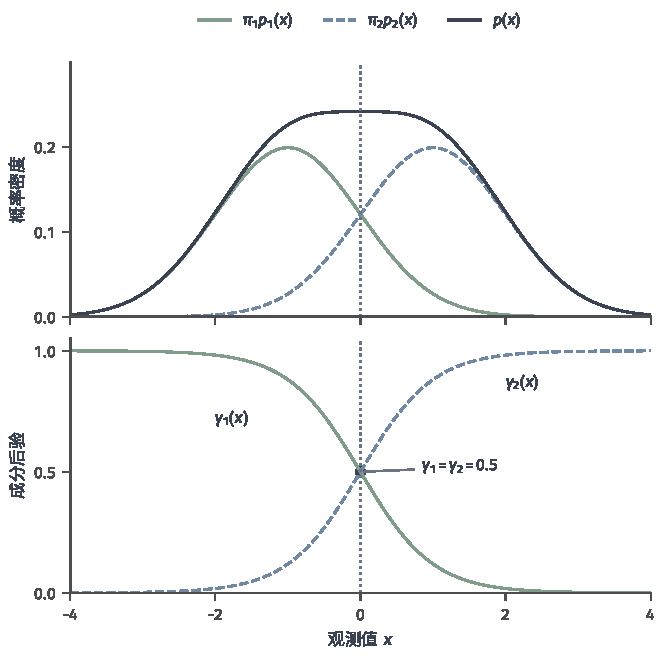
\includegraphics[width=105.412mm]{figures/04-classic-models/00-shared/matplotlib/clustering-gmm-responsibilities/figure.pdf}
  \caption{两成分 GMM 的密度与软归属。设 $\pi_1=\pi_2=1/2$、$\mu_1=-1$、$\mu_2=1$，两个方差均为 1，$p_k(x)$ 表示第 $k$ 个高斯密度。上图展示加权成分密度及其和，下图展示同一观测值对应的后验；颜色与线型在两图中保持一致。}
 \label{fig:clustering-gmm-responsibilities}
\end{figure}

\subsubsection{参数学习}

\term{期望最大化}（Expectation-Maximization, EM）交替估计潜在成分变量的分布和优化参数，Dempster、Laird 与 Rubin 将这一原则统一为一般框架\scite{clust-dempster1977}。E 步用当前参数 $\bm{\theta}^{(t)}$ 计算式~\eqref{eq:clustering-responsibility}；M 步固定这些责任度，最大化完全数据对数似然的期望。潜在成分变量不再藏在对数的求和中，而是通过 E 步给出的分布参与加权。

忽略与参数无关的常数，M 步目标为
\begin{equation}
 \begin{aligned}
 Q(\bm{\theta}\mid\bm{\theta}^{(t)})
 =\sum_{i,k}\gamma_{i,k}^{(t)}
 \biggl[&\log\pi_k-\frac12\log\det\bm{\Sigma}_k\\
 &-\frac12(\bm{x}_i-\bm{\mu}_k)^\top
 \bm{\Sigma}_k^{-1}(\bm{x}_i-\bm{\mu}_k)\biggr].
 \end{aligned}
 \label{eq:clustering-gmm-q}
\end{equation}
记有效样本量 $n_k^{(t)}=\sum_i\gamma_{i,k}^{(t)}$。权重优化加入约束 $\sum_k\pi_k=1$ 的拉格朗日乘子，驻点满足 $n_k^{(t)}/\pi_k=\lambda$；求和得到 $\lambda=n$，所以
\begin{equation}
 \pi_k^{(t+1)}=\frac{n_k^{(t)}}{n},\qquad
 \bm{\mu}_k^{(t+1)}
 =\frac{\sum_i\gamma_{i,k}^{(t)}\bm{x}_i}{n_k^{(t)}}.
 \label{eq:clustering-gmm-mean}
\end{equation}
均值公式来自 $Q$ 对 $\bm{\mu}_k$ 的梯度为零：公共正定因子 $\bm{\Sigma}_k^{-1}$ 消去，剩下加权残差和为零。

再令精度矩阵 $\bm{\Lambda}_k=\bm{\Sigma}_k^{-1}$，加权散布为
\[
 \bm{S}_k=\sum_i\gamma_{i,k}^{(t)}
 (\bm{x}_i-\bm{\mu}_k^{(t+1)})
 (\bm{x}_i-\bm{\mu}_k^{(t+1)})^\top.
\]
相关目标为 $\tfrac12[n_k^{(t)}\log\det\bm{\Lambda}_k-\operatorname{tr}(\bm{\Lambda}_k\bm{S}_k)]$。求导得 $n_k^{(t)}\bm{\Lambda}_k^{-1}-\bm{S}_k=\bm{0}$，于是
\begin{equation}
 \bm{\Sigma}_k^{(t+1)}
 =\frac{\bm{S}_k}{n_k^{(t)}}.
 \label{eq:clustering-gmm-covariance}
\end{equation}
更新要求有效样本量为正。加权散布正定时，无约束协方差取得正定域内的有限最优；退化散布则需要协方差约束或其他估计。

代码~\ref{code:clustering-gmm}在对数域计算责任度，并用协方差特征值下界$\epsilon$避免塌缩。该截断求解固定约束$\bm{\Sigma}_k\succeq\epsilon\bm{I}$下的M步；每轮任意加常数矩阵则对应另一种估计，需另说明目标。

\begin{codeblock}[language=Python,label={code:clustering-gmm}]{带协方差下界的 GMM--EM}
import numpy as np
from scipy.special import logsumexp
from scipy.stats import multivariate_normal

def gmm_em(X, K, max_iter=100, tol=1e-5, eps=1e-6):
    X = np.asarray(X, dtype=float)
    n, d = X.shape
    if eps <= 0:
        raise ValueError("eps must be positive")
    _, mu = kmeans(X, K)
    pi = np.full(K, 1.0 / K)
    cov = np.repeat((max(1., eps) * np.eye(d))[None], K, axis=0)
    def e_step():
        log_p = np.column_stack([
            np.log(pi[k]) + multivariate_normal.logpdf(
                X, mean=mu[k], cov=cov[k])
            for k in range(K)])
        normalizer = logsumexp(log_p, axis=1)
        gamma = np.exp(log_p - normalizer[:, None])
        return gamma, normalizer.sum()
    gamma, ll = e_step()
    for _ in range(max_iter):
        nk = gamma.sum(0)
        if (nk <= 0).any():
            raise ValueError("numerically empty component")
        pi = nk / n
        mu = (gamma.T @ X) / nk[:, None]
        for k in range(K):
            diff = X - mu[k]
            S = (diff * gamma[:, k, None]).T @ diff / nk[k]
            values, vectors = np.linalg.eigh(S)
            cov[k] = (vectors * np.maximum(values, eps)) @ vectors.T
        gamma, new_ll = e_step()
        if abs(new_ll - ll) <= tol * (1 + abs(ll)):
            break
        ll = new_ll
    return pi, mu, cov, gamma
\end{codeblock}

该实现调用前文的 K-means，以其中心初始化，返回的责任度由最终参数重新计算。协方差特征值截断之所以是上述受限 M 步的解，是因为最优协方差与加权散布共享特征向量，每个特征值分别最小化 $\log s+\lambda/s$，在 $s\geq\epsilon$ 上得到 $s=\max\{\lambda,\epsilon\}$。计算中可同时记录似然变化、不同重启的目标和近空成分，以检查数值误差及初始化影响。

完整协方差保留全部二阶方向关系；类内有效样本不足时，可采用对角、球形或共享协方差减少自由度。完整形式一轮约需$O(nKd^2+Kd^3)$运算，立方项来自矩阵分解，对角形式的主要成本为$O(nKd)$。K-means++、重启和初始划分协方差可提供不同起点，其结果在同一约束与似然下比较。

\subsubsection{理论分析}

\paragraph{表达能力}
GMM用有限个高斯分量的混合表达密度。分量数、协方差限制与参数范围决定自由度；一个语义类别可以需要多个分量，一个分量也不能预先当作真实类别。

\paragraph{收敛性}
EM在旧参数处构造与观测似然相等的下界，再提高这一辅助目标。这样可避免直接优化对数内的成分求和；精确E步与M步改进条件共同给出似然不下降。

\begin{theorem}[EM 的似然单调性]
 \label{thm:clustering-em}
 E 步取当前精确后验，M 步满足
 $Q(\bm{\theta}^{(t+1)}\mid\bm{\theta}^{(t)})
 \geq Q(\bm{\theta}^{(t)}\mid\bm{\theta}^{(t)})$。
 在相关概率与期望有限、支持条件允许下，则
 $\ell(\bm{\theta}^{(t+1)})\geq\ell(\bm{\theta}^{(t)})$。
\end{theorem}
\begin{proof}
对每个样本，令$q_i$相对于当前参数下成分后验的KL散度有限，直接使用整体对数比形式（参考\BookSectionRef{sec:information-elbo-approximation}{第一卷“数学准备”的“表示约束下的分布逼近”小节}）：
\[
 \begin{aligned}
 \mathcal L_i(q_i,\bm\theta)
 &=\sum_{k:q_i(k)>0}q_i(k)
    \log\frac{p(\bm x_i,z_i=k;\bm\theta)}{q_i(k)},\\
 \log p(\bm x_i;\bm\theta)
 &=\mathcal L_i(q_i,\bm\theta)
   +D_{\mathrm{KL}}\bigl(q_i\Vert p(z_i\mid\bm x_i;\bm\theta)\bigr).
 \end{aligned}
\]
对样本求和，把下界记为$\mathcal L(q,\bm\theta)$。该分解不要求$q_i$覆盖后验的全部支撑；
若改用恢复证据的Jensen等式，则必须另查相反方向的覆盖条件。
E 步令 $q_i^{(t)}$ 等于旧参数的后验，因此 $\mathcal{L}(q^{(t)},\bm{\theta}^{(t)})=\ell(\bm{\theta}^{(t)})$。固定 $q^{(t)}$ 后，下界与 $Q$ 仅相差不含参数的熵项，M 步遂给出
\[
 \begin{aligned}
 \ell(\bm{\theta}^{(t+1)})
 &\geq\mathcal{L}(q^{(t)},\bm{\theta}^{(t+1)})\\
 &\geq\mathcal{L}(q^{(t)},\bm{\theta}^{(t)})
 =\ell(\bm{\theta}^{(t)}).
 \end{aligned}
\]
这就证明了单调性。
\end{proof}

似然有上界时，EM的单调性可进一步给出似然值收敛。参数趋于驻点还需连续性、紧性等正则条件，Wu给出了相应分析\scite{clust-wu1983}。驻点可能是局部极大值或鞍点，优化解释应分别核对值的极限、参数极限和驻点类型。

当 $K\geq2$，且模型中存在一个可塌缩的正权重成分，其余正权重成分仍使其他样本的混合密度保持正值时，无约束 GMM 的似然没有上界。令可塌缩成分的均值等于某个样本，协方差为 $\sigma^2\bm{I}$；当 $\sigma\to0$ 时，该样本处的密度按 $\sigma^{-d}$ 增长，而其他样本仍由其余成分覆盖，因此总对数似然可以无界增加。若 $K=1$ 且样本经验散布矩阵正定，单高斯的最大似然有限；若经验散布矩阵奇异，协方差仍可能在数据未占据的方向趋近边界并导致似然退化。协方差下界、适当先验或惩罚可以阻止这类塌缩，但它们各自改变了优化问题。

潜在成分编号的置换不改变混合密度；当成分彼此不同且权重为正时，一个解通常对应 $K!$ 个等价标号。这与不同拟合质量的局部极值是两类问题。

\paragraph{泛化性}
新样本平均对数似然评价预测密度，训练似然描述经验拟合。成分数与协方差形式改变拟合能力，也改变估计所需样本；信息准则在同一约束下比较这种取舍。完整协方差的参数数目为
\[
 m_K=(K-1)+Kd+\frac{Kd(d+1)}{2},
\]
常用准则为
\begin{equation}
 \mathrm{BIC}(K)=-2\ell(\hat{\bm{\theta}}_K)+m_K\log n,
 \qquad
 \mathrm{AIC}(K)=-2\ell(\hat{\bm{\theta}}_K)+2m_K.
 \label{eq:clustering-bic}
\end{equation}
两个准则以惩罚参数量后的拟合选择候选，取较小值。BIC的证据近似需要渐近条件，而有限混合包含零权重边界、不可辨识和奇异参数。应用于混合阶数时，应核对专门的一致性条件\scite{clust-keribin2000}。

混合阶数说明所选分布族拟合数据需要多少成分。将其解释为语义类别数，还需外部知识或验证表明一个类别与一个成分对应。

\subsubsection{小结}

GMM以软后验、协方差与预测密度支持概率聚类，也可用于语音建模和异常评分。分布失配、似然奇异与局部求解影响估计；增加高斯成分可改善密度表达，同时增加解释每个成分的负担。

\subsection{模型对比与总结}

GMM的软归属、权重与协方差共同定义后验，K-means只使用中心平方距离。固定部分参数并取小方差极限，可以明确两种目标和更新的联系。固定均匀权重 $\pi_k=1/K$ 和共享球形协方差 $\bm{\Sigma}_k=\sigma^2\bm{I}$，则
\[
 \gamma_{i,k}=
 \frac{\exp(-\lVert\bm{x}_i-\bm{\mu}_k\rVert_2^2/(2\sigma^2))}
 {\sum_j\exp(-\lVert\bm{x}_i-\bm{\mu}_j\rVert_2^2/(2\sigma^2))}.
\]
若 $\bm{x}_i$ 的最近中心唯一为 $k^\ast$，则对任意 $j\ne k^\ast$，距离平方差为正，相应指数比随 $\sigma^2\to0$ 趋零，故 $\gamma_{i,k^\ast}\to1$。M 步的均值更新因此退化为 Lloyd 更新；平局时责任度可分散在多个最近中心，不能直接得到唯一硬簇分配。

去掉只依赖$\sigma$的常数，目标$-2\sigma^2\ell$趋向$\sum_i\min_k\lVert\bm{x}_i-\bm{\mu}_k\rVert_2^2$，给出平方误差的联系。这一极限固定均匀权重并缩小共享球方差；自由协方差GMM优化更大的分布族。FCM的软隶属度则来自模糊损失，与生成后验采用不同定义。

更换成分分布即可适配其他数据：伯努利混合适合二值特征，多项式混合适合计数向量；重尾的 $t$ 混合可减轻离群观测对均值和尺度估计的影响，其代价是引入额外的尺度或自由度估计\scite{clust-peel2000}。

\term{狄利克雷过程混合}（Dirichlet process mixture, DPM）为随机混合分布设置Dirichlet过程先验，使潜在成分数随数据和后验变化。总质量参数控制新增成分的倾向，折棒表示及后验预测见第\ref{sec:pgm-static-directed-hierarchy-membership}节；Neal研究了相应MCMC推断\scite{clust-neal2000}。模型省去固定$K$，仍需选择先验并核对潜在成分与任务类别的关系。

概率路线在同一生成模型下计算归属、预测密度和模型比较。所需输出及分布假设决定是否采用它；与几何或密度方法比较时，还需先确定共同的使用目标。

\section{基于集成的聚类}
\label{sec:clustering-ensemble}

不同初始化、表示或算法可能在同一批对象上产生多份划分。\term{共识聚类}（consensus clustering）统计每对对象在多少份划分中共簇，形成共关联矩阵，再聚类该矩阵或对应图\scite{clust-strehl2002}。这一机制把候选间的共同结构汇为一个新输入，也可用于诊断反复出现的群组。

直接比较共关联矩阵要求对象集固定。重采样改变对象集时，可只比较共同对象，或先冻结新样本分配规则，再将候选应用到相同评价对象；协议见表\ref{tab:clustering-evaluation-protocol}。独立样本没有共同对象时，应预定候选生成方式，改为比较簇轮廓、外部关联或用途指标。

共识本身仍由候选产生。同一数据上的反复筛选不会补充外部验证，多数划分也可能淹没少数有意义的结构。报告时应保留共关联强度、候选来源，以及在独立评价中相对无聚类基线的收益。

\section{半监督聚类}
\label{sec:clustering-semisupervised}

未标注数据也可能附有部分领域知识。例如，专家知道两条记录来自同一对象，知道一对样本应分开，或能给出少量典型种子。\term{半监督聚类}（semi-supervised clustering）将这些信号用于以未标注样本为主体的分组。

第\ref{sec:classification-semisupervised}节的半监督分类利用未标注输入改进预先定义类别的预测，本节则用少量类别标签或关系先验共同决定分组。两者都改变可用监督信息，却保留不同的任务目标。

实例级信号常写为\term{必连约束}（must-link）和\term{勿连约束}（cannot-link）：前者要求两个样本同簇，后者要求异簇。记其索引对集合为 $M$ 和 $B$，以免与簇 $C_k$ 或划分 $\mathcal{P}$ 混淆。信号既可作为硬约束，也可带权违反；少量关系判断是否比逐点类别标签更容易获取，取决于实际标注任务。

这些信号与几何结构共同确定群组。需要检验的是先验是否消除了原模型的歧义，覆盖了哪些样本，以及是否与基础几何发生冲突；信号质量和作用范围决定其可能收益。

\subsection{COP-K-means}
\label{sec:clustering-cop}

关系被视为硬事实时，分配必须避开与它们冲突的簇。Wagstaff等在2001年提出COP-K-means，将最近中心选择限制在当前可行选项内\scite{clust-wagstaff2001}。这既改变候选分配，也引入可行性与访问顺序问题。

\subsubsection{模型结构}

目标仍为式~\eqref{eq:clustering-sse}，可行域增加
\begin{equation}
 c_i=c_j\quad((i,j)\in M),\qquad
 c_i\ne c_j\quad((i,j)\in B).
 \label{eq:clustering-cop}
\end{equation}
must-link 的传递闭包把样本分成\term{约束块}（chunklet），同一块必须整体分配。若 cannot-link 的两端落在同一块内，约束立即矛盾；但不存在这种矛盾还不足以保证给定 $K$ 下可行。

把每个约束块当作顶点、cannot-link 当作边，块的簇分配实际上是该图的 $K$ 着色。例如三个两两 cannot-link 的块不能放进两个簇，即使没有任何 must-link 冲突。块级 SSE 可分解为块内常数加上“块大小乘以块均值到中心的平方距离”，因此整体分配也能利用摘要。

\subsubsection{参数学习}

COP-K-means 按某个顺序处理样本或约束块，对候选簇按距离排序，接受第一个与已固定分配相容的簇。若没有候选，就报告本次贪心分配失败；更新步则对每个非空簇取均值。

\begin{algorithm}[COP-K-means 的约束块分配]
 \label{alg:clustering-cop}
 \begin{algorithmic}[1]
 \Require must-link 闭包、块间 cannot-link、当前中心
 \Ensure 本轮可行分配，或本轮贪心失败
 \State 清空本轮簇分配，选定约束块访问顺序
 \For{每个约束块 $U$}
  \State 按 $\sum_{i\in U}\lVert\bm{x}_i-\bm{\mu}_k\rVert_2^2$ 排序候选簇
  \State 选择不与已分配邻块冲突的最近候选
  \If{候选不存在}
   \State 返回本轮失败
  \EndIf
  \State 把 $U$ 的全部样本分给所选簇
 \EndFor
 \end{algorithmic}
\end{algorithm}

贪心失败可能来自顺序，而非约束本身。以cannot-link路径$a-b-c-d$和$K=2$为例：按$a,d,b,c$访问，若$a,d$先取簇1，$b$只能取簇2，$c$便无可行选择。整体划分$\{a,c\}$与$\{b,d\}$却满足全部关系，说明局部已定选择阻碍了后续分配。

逐块贪心未精确求解固定中心的整体约束分配，Lloyd的下降前提在这里需要重新建立。可从已有可行解出发，只接受可行且降低目标的块移动；也可精确求解受约束分配，再更新均值。前者搜索范围较小，后者增加组合优化成本。普通COP实现可用迭代上限、失败记录及重启或回溯处理这些情况。

\subsubsection{小结}

COP-K-means 的好处是约束含义明确，成功输出可以逐项检查是否满足关系。代价是约束冲突、给定 $K$ 下不可行以及贪心顺序失败都必须处理。若先验允许出错，PCK-means 在 SSE 上增加
\[
 \sum_{(i,j)\in M}w_{i,j}^{M}\mathbb{1}\{c_i\ne c_j\}
 +\sum_{(i,j)\in B}w_{i,j}^{B}\mathbb{1}\{c_i=c_j\},
\]
以软惩罚权衡几何和约束。有限权重不保证零违反，但避免因单条错误关系直接拒绝整个问题。

\subsection{Seeded / Constrained K-means}
\label{sec:clustering-seeded}

若已知的是少量样本的类别名称，可以直接用它们确定初始中心或固定归属。Basu、Banerjee 与 Mooney 在 2002 年研究了 Seeded K-means 与类别标签约束的 Constrained K-means\scite{clust-basu2002}。后者与第~\ref{sec:clustering-capacity} 节的同名容量约束方法含义不同：本节锁定种子的类别标签，容量方法限制各簇样本数。

\subsubsection{模型结构}

设种子索引集合为 $S$，类别标签为 $\ell_s\in\{1,\ldots,K\}$，并记 $S_k=\{s\in S:\ell_s=k\}$。当每类都有种子时，初始化为
\[
 \bm{\mu}_k^{(0)}
 =\frac{1}{|S_k|}\sum_{s\in S_k}\bm{x}_s.
\]
缺少种子的簇需另外初始化。Seeded 版本只在初始化时使用类别标签，之后种子可以移动；Constrained 版本始终要求 $c_s=\ell_s$，把种子类别标签作为硬事实。二者都优化同一个平方误差目标，只是初始化与可行域不同。

\subsubsection{参数学习}

Seeded 版本随后直接运行 Lloyd。Constrained 版本在分配步冻结种子，其余样本独立选择最近中心；更新中心时同时计入种子和非种子。由于冻结限制彼此不耦合，逐点分配仍是固定中心下的精确最优解，因此可沿用定理~\ref{thm:clustering-lloyd} 的下降论证与平局条件。每簇都有固定种子时，还自然避免了空簇。

种子确定了部分群组的名称与初始位置，其代表性仍影响结果。允许种子移动，可以缓解错误标签的永久锁定；可靠标签与模糊几何并存时，冻结种子更能保留监督关系。选择哪种方式，应按种子覆盖、比例和错误类型，在未参与拟合的证据上比较。

\subsubsection{小结}

种子方法通过初始化或固定归属引入少量类别标签，适合每类已有代表样本的任务。距离与均值继续规定几何；若监督还需改变特征方向的重要性，可以进一步学习度量。

\subsection{MPCK-means}
\label{sec:clustering-mpck}

如果重要特征与无关特征混在一起，约束即使改变了簇分配，也未必能改变下一轮的距离判断。Bilenko、Basu 与 Mooney 在 2004 年提出的 MPCK-means（Metric Pairwise Constrained K-means）同时优化分配和簇相关度量，使关系约束既影响簇分配，也影响空间中的方向与尺度\scite{clust-bilenko2004}。

弱监督可以进入不同环节：关系限制可行分配，种子确定初始位置或成员，成对约束还可学习方向与尺度。这些形式对应不同的先验内容和可信程度，可按信号实际支持的判断选择。

\subsubsection{模型结构}

为簇 $k$ 配置正定矩阵 $\bm{A}_k\succ0$，定义平方 Mahalanobis 距离
\[
 d_{\bm{A}_k}^2(\bm{x},\bm{y})
 =(\bm{x}-\bm{y})^\top\bm{A}_k(\bm{x}-\bm{y}).
\]
正定性既保证非退化距离，也使 $\log\det\bm{A}_k$ 有定义。可以把这种距离看作先做坐标变换 $\tilde{\bm{x}}=\bm{A}_k^{1/2}\bm{x}$，再计算欧氏距离。图~\ref{fig:clustering-metric-constraints} 给出了一个固定变换的例子：压缩水平方向、拉伸竖直方向后，must-link 对变近，而 cannot-link 对变远。实际 MPCK-means 需要根据全部样本与约束优化 $\bm{A}_k$，并非预先知道图中的变换。

\begin{figure}[htbp]
  \centering
  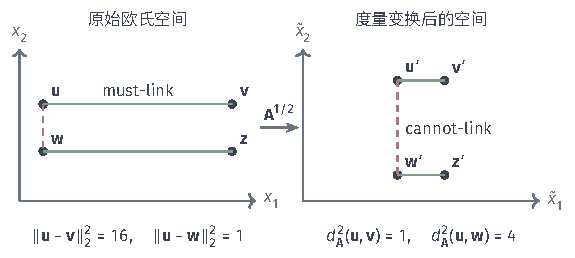
\includegraphics[width=97.331mm]{figures/04-classic-models/00-shared/tikz/clustering-metric-constraints/figure.pdf}
  \caption{度量如何改变成对关系的几何表达。四点为 $\bm{u}=(-2,0.5)$、$\bm{v}=(2,0.5)$、$\bm{w}=(-2,-0.5)$、$\bm{z}=(2,-0.5)$。实线连接 must-link 对，虚线连接 cannot-link 对。这里人为设定 $\bm{A}=\operatorname{diag}(1/16,4)$；右图的距离等于左图的 Mahalanobis 距离，不表示一次真实训练的结果。}
 \label{fig:clustering-metric-constraints}
\end{figure}

记在该度量下全数据的最大距离平方为
\[
 D_k=\max_{p,q\in\{1,\ldots,n\}}
 d_{\bm{A}_k}^2(\bm{x}_p,\bm{x}_q).
\]
对违反 must-link 的样本对，惩罚同时作用于两端所属簇；对违反 cannot-link 的样本对，惩罚其相对于本簇度量下最远样本对的接近程度。具体写为
\begin{align}
 f_M(i,j)
 &=\frac12\left[
 d_{\bm{A}_{c_i}}^2(\bm{x}_i,\bm{x}_j)
 +d_{\bm{A}_{c_j}}^2(\bm{x}_i,\bm{x}_j)\right]
 \mathbb{1}\{c_i\ne c_j\},\nonumber\\
 f_B(i,j)
 &=\left[D_{c_i}
 -d_{\bm{A}_{c_i}}^2(\bm{x}_i,\bm{x}_j)\right]
 \mathbb{1}\{c_i=c_j\}.
 \label{eq:clustering-mpck-penalty}
\end{align}
因此 cannot-link 惩罚非负，must-link 惩罚也不因交换样本对的书写顺序而改变。总目标为
\begin{equation}
 \begin{aligned}
 J={}&\sum_{k=1}^K\sum_{i\in C_k}
 \left[d_{\bm{A}_k}^2(\bm{x}_i,\bm{\mu}_k)
       -\log\det\bm{A}_k\right]\\
 &+\sum_{(i,j)\in M}w_{i,j}^{M}f_M(i,j)
  +\sum_{(i,j)\in B}w_{i,j}^{B}f_B(i,j).
 \end{aligned}
 \label{eq:clustering-mpck}
\end{equation}
权重均非负，每个无序约束对只计一次。负对数行列式阻止特征值趋零，但不能单独阻止矩阵某些方向无限放大；数据退化时仍需约束或正则。

\subsubsection{参数学习}

固定中心和度量时，对一个样本的各簇候选计算完整目标变化，包括几何、行列式及所有相关关系惩罚，再接受不增目标的变更。由于关系项耦合样本，单独比较到中心的距离不足以完成这项选择。

固定分配和度量时，约束项不含中心。对中心求导给出
\[
 2\bm{A}_k\sum_{i\in C_k}(\bm{\mu}_k-\bm{x}_i)=\bm{0},
 \qquad
 \bm{\mu}_k=\frac{1}{|C_k|}\sum_{i\in C_k}\bm{x}_i.
\]
同一簇共用的$\bm{A}_k$在驻点方程中消去，中心因而取普通簇内均值。若需按样本重要性加权，还要在目标中另加相应权重。

度量步可借助散布矩阵理解。令 $\bm{S}_k=\sum_{i\in C_k}(\bm{x}_i-\bm{\mu}_k)(\bm{x}_i-\bm{\mu}_k)^\top$。在固定当前最远样本对、且该样本对在更新后仍保持活跃的一个分支上，约束项写成 $\operatorname{tr}(\bm{A}_k\bm{P}_k)$，其中 $\bm{P}_k$ 汇总违反 must-link 的半权重差分外积，以及违反 cannot-link 的“最远对外积减约束对外积”。于是子目标为
\[
 \operatorname{tr}\bigl(\bm{A}_k(\bm{S}_k+\bm{P}_k)\bigr)
 -|C_k|\log\det\bm{A}_k.
\]
若 $\bm{S}_k+\bm{P}_k\succ0$ 且 $|C_k|>0$，其无约束驻点为
\begin{equation}
 \bm{A}_k=|C_k|(\bm{S}_k+\bm{P}_k)^{-1}.
 \label{eq:clustering-mpck-metric}
\end{equation}
这个驻点式适用于正定的调整散布及保持活跃的最远对分支；更新后需再次核对这两个条件。

保留 $D_k$ 对 $\bm{A}_k$ 的真实依赖时，它是有限个线性函数的最大值，故固定分配和中心的度量子问题是凸的，但通常分段光滑。可在 $\alpha\bm{I}\preceq\bm{A}_k\preceq\beta\bm{I}$、$0<\alpha<\beta$ 的固定域上求解，或使用保持正定且实际下降的优化步骤。对角度量进一步减少参数与矩阵计算。

各步在同一有下界的目标上不增，可推出目标值收敛。度量属于连续参数，即使簇分配不再变化，它也可能继续更新；有限分配数因此不足以证明有限轮停止。实际终止可结合目标和参数变化的容差，并明确空簇处理。

\subsubsection{小结}

MPCK-means用成对监督调整几何，同时估计分配与每簇度量。ITML、LMNN也学习度量，但采用不同损失和训练约束，相关工具需按目标分别使用。每簇完整矩阵有$d(d+1)/2$个自由参数，监督较少或维数较高时可共享或取对角，以降低估计容量。

\subsection{模型对比与总结}

COP限制实例关系，种子方法引入类别名称，MPCK-means将关系用于学习几何。硬约束要求输出完全满足，软权重则允许以违反换取其他拟合收益。选择前应明确信号的可信程度与覆盖；增加度量参数还需要足够监督支持。下面再比较信号进入图与共享度量的方式。

先验也可加入谱聚类。Kamvar、Klein 与 Manning 的 Spectral Learning 研究了将监督信息纳入谱表示；一种直接做法是提高 must-link 边权、降低 cannot-link 边权，再对修改后的非负对称图求谱表示\scite{clust-kamvar2003}。

边权调整改变谱偏好，最终分配仍由整张图和离散化决定。即使删除cannot-link边，两端也可能通过其他强边共簇。修改后的非负对称图可按其新拉普拉斯分析，但谱间隙、连接及统计条件需重新核对。关系传播还能扩展局部监督，同时可能扩散错误信号。

Xing 等通过相似与不相似样本关系学习 Mahalanobis 度量\scite{clust-xing2003}。这是先单独学习共享度量、再交给聚类算法的解耦方式。这样可以复用监督得到的几何结构，但共享度量仍假设所有簇使用同一种空间变换，后续算法也须与该度量兼容。

半监督聚类应评价先验是否解决了原模型无法区分的选择。可同时报告几何目标、关系违反，以及独立参考标签或下游任务中的结果；训练关系的满足度描述监督拟合，独立评价再检查其用途与泛化。

\section{模型选择与评价}
\label{sec:clustering-evaluation}

\subsection{方法比较}

原型方法比较样本与代表的相异度，邻域和图方法从局部连通关系形成群组，网格与子空间方法改变比较单位，层次方法保留多个粒度，概率方法解释软归属，集成则汇总多份分组。表\ref{tab:clustering-navigation}对照这些簇判据及输出条件；HDBSCAN等方法可以同时涉及邻域与层次。

\begin{table*}[htbp]
  \centering
  \small
  \begin{tabularx}{\linewidth}{@{}>{\RaggedRight\arraybackslash}p{22mm}*{5}{>{\RaggedRight\arraybackslash}X}@{}}
    \toprule
    代表方法 & 簇判据 & 输出粒度 & 表示或相异度 & 优化或推断机制 & 监督信息 \\
    \midrule
    K-means、K-medoids & 到原型的总相异度 & 给定$K$的平坦硬划分 & 数值向量上的平方距离；一般对象相异度 & 交替更新；代表交换 & 无 \\
    DBSCAN、OPTICS、HDBSCAN、Mean Shift & 密度连通或模态吸引域 & 噪声、排序、层次或模态簇 & 邻域距离或核密度 & 区域扩展、排序、树压缩或模态搜索 & 无 \\
    谱聚类、AP、Louvain & 图割、代表支持或模块度 & 平坦划分；簇数可显式或间接控制 & 原生图或由相似度构造的加权图 & 特征松弛、消息传递或局部移动 & 无 \\
    STING、CLIQUE、投影聚类 & 密集单元或低维紧凑性 & 区域、重叠子空间或硬划分 & 网格、坐标子集或学习的投影 & 摘要查询、候选搜索或代表迭代 & 无 \\
    AGNES、DIANA & 链接或分裂准则 & 嵌套层次，事后截取 & 点或簇间相异度 & 贪心合并或启发式分裂 & 无 \\
    GMM、DPM & 生成成分及其后验 & 平坦软归属；成分数固定或随机 & 数值向量及指定分布族 & EM、MCMC或变分推断 & 先验不等同于类别标签 \\
    共识聚类 & 多份分组的共同结构 & 通常为平坦划分 & 共簇关系或超图 & 共识函数、图划分等 & 依赖成员所用信息 \\
    COP、Seeded、MPCK-means & 基础簇判据加关系或种子约束 & 通常为平坦硬划分 & 原始或学习的度量、约束图 & 受限分配、初始化或度量学习 & 成对关系、种子或少量类别标签 \\
    \bottomrule
  \end{tabularx}
  \caption{聚类方法的属性导航。每行登记代表方法在五项属性上的基本设定，不把各主体节解释成互斥类别；方法的具体变体可能改变其中一项或多项。}
  \label{tab:clustering-navigation}
  \label{tab:clustering-overview}
\end{table*}

\subsection{评价与选择}

\paragraph{表示与相异度}
客户变量的类型与尺度先规定可比较的相异度。测量协议可以预定尺度，也可以从数据估计标准化；后一种做法改变各坐标在距离中的权重，需要对应任务含义。类别变量可比较取值是否相同，序数变量还需说明等级间距。

数值与类别混合时，可将每个变量的相异度变到可比范围，再按给定权重汇总。Gower系数采用这一构造，对每个样本对只使用共同观测的变量，并按对应权重归一化\scite{clust-gower1971}。数据估计的尺度、插补、范围和权重在下文的发现数据上拟合，再冻结用于验证。

索引或近似算法若使用三角不等式，需要确认所选相异度满足它。图方法还需规定单向近邻的对称化、边权缩放与孤立点处理。这些规则改变距离或连接，也会改变“同一簇”的具体含义。

\paragraph{发现与验证}
算法停止、目标值收敛和参数收敛描述计算；训练外是否出现有用群组则是验证问题。为分别获得这两种证据，可划分\term{发现数据}（discovery data）与\term{验证数据}（validation data）。发现数据用于估计表示、尺度和相异度，拟合候选并选择簇数或超参数；查看验证结果前，固定方法、簇匹配、指标及用途判断。

验证数据可来自同源留出或独立收集。时间、地点和个体相关数据应按未来使用单位划分，减少相关记录跨集合带来的泄漏。Ullmann、Hennig与Boulesteix系统讨论了复核聚类的验证方式\scite{clust-ullmann2022}。

表\ref{tab:clustering-evaluation-protocol}按问题安排六种证据。训练目标、稳定性和零模型可在发现阶段用于诊断；独立外部标签检验指定语义，留出拟合与下游效用检验样本外用途。候选较多时，可在发现数据内部嵌套划分或交叉验证，将最终验证保留到规则固定之后。

稳定性测量重采样或参数变化的影响，也受目标唯一性和数据对称性控制\scite{clust-ben-david2006}。解释它时，还需核对簇含义与用途。零模型则规定“没有所关心结构”时保留哪些数据特征；Gap Statistic将观测簇内离差与参考分布比较，是其中一种构造\scite{clust-tibshirani2001-gap}。

校准零模型证据时，每份模拟数据都应重跑与观测数据相同的完整流程，包括预处理、拟合、候选搜索及选择。这样才将选择本身的影响纳入参考分布；仅固定某一结果再模拟，可作为探索基线，证据对象相应较窄。

内部指标解释当前拟合，也带有自身的几何偏好。SSE评价中心量化，\term{轮廓系数}（silhouette coefficient）比较同簇平均距离与最近其他簇平均距离，评价相对紧凑程度\scite{clust-rousseeuw1987}。跨方法比较时，应先确认这种几何与共同目标相符。

\term{调整兰德指数}（adjusted Rand index, ARI）比较同一批对象在两份划分中的共簇与异簇关系，并在固定簇大小的随机划分下校正期望一致性\scite{clust-hubert1985}。它对簇编号置换不变，可比较重复运行，也可比较独立参考标签。后者检验指定外部语义，其他合理群组仍需不同证据。

\begin{table*}[htbp]
  \centering
  \small
  \begin{tabularx}{\linewidth}{@{}>{\RaggedRight\arraybackslash}p{21mm}>{\RaggedRight\arraybackslash}p{43mm}>{\RaggedRight\arraybackslash}X>{\RaggedRight\arraybackslash}X@{}}
    \toprule
    证据 & 最小执行协议 & 可以回答 & 不能单独推出 \\
    \midrule
    训练目标 & 在发现数据上记录SSE、似然、图目标或约束违反，并只与相同目标和约束下的候选比较 & 求解是否满足方法声明的经验准则 & 语义正确、跨目标优越或样本外有效 \\
    稳定性 & 对象集固定而只改变测量、初始化或关键参数时，比较共簇关系或标签置换不变的分区指标；样本重采样改变对象集时，只比较共同对象，或冻结新样本分配规则后再比较 & 哪些群组依赖少量样本、随机性或参数 & 正确簇数或业务语义；稳定性本身也可能来自唯一目标或数据对称性 \\
    外部标签 & 标签不参与无监督拟合与选择；在验证数据上按预先规定的总体或子群计算ARI等指标 & 与指定外部语义的一致程度 & 标签之外的其他合理结构，或无标签任务中的唯一真解 \\
    零模型 & 先说明要保留的边际、范围或相关结构；在每份模拟数据上重跑相同的预处理、拟合、候选搜索和选择规则；未重跑完整管线时只作为探索性基线 & 观察到的分离是否超出该无簇基线；Gap Statistic是一个实例 & 拒绝所有其他零模型，或证明所得簇具有用途 \\
    留出证据 & 用发现数据拟合表示和模型，按冻结的新样本分配规则评价留出量化误差或预测对数密度 & 指定模型在同一数据制度下的样本外拟合 & 不同簇概念之间的统一优劣；无样本外规则的方法须先定义映射 \\
    下游效用 & 冻结簇提取流程，在嵌套验证中与无聚类或更简单基线比较检索、描述或决策损失 & 群组是否改善预先声明的实际用途 & 群组在其他用途或总体上仍然有效 \\
    \bottomrule
  \end{tabularx}
  \caption{聚类结果的评价协议。发现阶段可以生成和筛选候选；最终验证数据只在表示、算法、超参数和比较规则冻结后使用。每类证据回答不同问题，指标的几何偏好和数据依赖必须随结果报告。}
  \label{tab:clustering-evaluation-protocol}
\end{table*}

不同证据可能支持不同结论。SSE更低而下游损失更高，说明量化目标与用途存在偏离；稳定性高但与零模型相近，说明重复出现的结构还缺少超出参考基线的证据；外部标签一致但预测密度较差，则提示标签与生成族可能不对应。

结论应对应预定群组和用途，同时保留这些差异。指标本身也偏好特定形状与粒度，Handl等的比较强调按验证问题选择证据\scite{clust-handl2005}。


聚类公理还依赖输出形式。Kleinberg对固定对象、成对距离输入与单一划分输出证明：尺度不变性、丰富性和一致性无法同时成立\scite{clust-kleinberg2002}。它揭示这一设定的要求冲突；软归属、重叠和层次使用其他输出约束。流式、多视图与神经聚类还改变数据或表示，其验证也需对应实际设定。

前述理论分别约束具体计算。Lloyd用下降和平局规则证明有限停止，Ward比较一次合并，DBSCAN固定核心点分量。Mean Shift和EM先给目标单调，再以附加条件讨论参数；谱松弛控制连续子问题，CLIQUE保证特定计数剪枝完整。实现时可用这些对象核对算法步骤，再另行检验样本外结构。

聚类扩展回应不同需求。样本规模推动小批量、抽样与摘要，以近似或顺序影响换取计算；非凸形状推动密度连通、核和谱，同时增加邻域与构图选择；关系输入使中心样本与图目标直接使用对象联系，也引入距离存储和图计算。

高维数据推动子空间与投影搜索，代价是组合候选和方向估计。概率语义带来软后验、预测密度及模型比较，同时需要处理分布失配、奇异性和局部推断。弱监督用关系或种子消除部分歧义，其覆盖不足和错误又可能影响多个样本。

这些变化处理不同压力，可组合使用。验证进一步检查所改机制是否带来预定收益，按零模型、重复性、独立数据及用途取得证据；方法的适用条件由这一问题链确定。

客户分群应先规定用途。量化关注表示误差，探索关注可重复结构，解释关注群组与外部语义，下游决策关注实际损失。用途确定后，再选择变量尺度、相异度或邻接、簇判据、输出粒度及可用先验。

快速数值量化可从K-means开始，真实代表与一般相异度可用K-medoids，多层解释可用层次树。低密度分隔和噪声识别可评价DBSCAN、OPTICS或HDBSCAN；关系数据先解释边权，再选择图目标。相关坐标因簇变化时可搜索子空间，概率输出重要时可拟合混合，已有可靠知识时可加入关系或种子。

候选确定后，按表\ref{tab:clustering-evaluation-protocol}取得相应证据：留出量化误差检验数值拟合，稳定性与零模型检验探索结构，独立关联检验语义，相对无聚类基线的损失检验决策收益。由此说明哪些客户、数据条件和用途支持当前分组。

\Needspace{18\baselineskip}
\section{本章小结}
\label{sec:clustering-summary}

聚类通过结构假设定义群组。原型限定中心周围的相异度，邻域和图限定连接，网格与子空间限定相关区域，层次限定嵌套关系，概率模型限定生成成分，集成汇总候选共同结构。关系与种子监督再减少其中部分歧义。

算法求解与群组用途需要不同证据。目标下降和停止支持计算解释，训练外量化、密度、语义或决策结果支持使用结论；稳定性及零模型补充结构检验。粒度由$K$、密度阈值、带宽、截线或先验控制，均需随任务选择。

第\ref{chap:dimensionality-reduction}章将学习低维表示，这会同时改变距离、密度和邻接。可视化提供探索线索，群组判断仍需在原始或经验证的表示上取得与用途对应的证据。

\paragraph{扩展阅读}
Bishop第9章从潜变量解释混合与EM，Hastie等在无监督学习中比较距离、原型及层次\scite{bishop2006,hastie2009}。进一步阅读可选同一数据问题，分别写出簇定义、迭代目标与新样本评价，比较不同假设怎样改变最终群组。